%	%
% Niniejszy plik stanowi przykład formatowania pracy magisterskiej na
% Wydziale MIM UW.  Szkielet użytych poleceń można wykorzystywać do
% woli, np. formatujac wlasna prace.
%
% Zawartosc merytoryczna stanowi oryginalnosiagniecie
% naukowosciowe Marcina Wolinskiego.  Wszelkie prawa zastrzeżone.
%
% Copyright (c) 2001 by Marcin Woliński <M.Wolinski@gust.org.pl>
% Poprawki spowodowane zmianami przepisów - Marcin Szczuka, 1.10.2004
% Poprawki spowodowane zmianami przepisow i ujednolicenie 
% - Seweryn Karłowicz, 05.05.2006
% Dodanie wielu autorów i tłumaczenia na angielski - Kuba Pochrybniak, 29.11.2016

% dodaj opcję [licencjacka] dla pracy licencjackiej
% dodaj opcję [en] dla wersji angielskiej (mogą być obie: [licencjacka,en])
\documentclass[licencjacka]{pracamgr}


% Dane magistranta:
\autor{Paweł Tomaszewski}{292647}


% Dane magistrantów:
%\autor{Autor Zerowy}{342007}
%\autori{Autor Pierwszy}{342013}
%\autorii{Drugi Autor-Z-Rzędu}{231023}
%\autoriii{Trzeci z Autorów}{777321}
%\autoriv{Autor nr Cztery}{432145}
%\autorv{Autor nr Pięć}{342011}

\title{Interaktywna eksploracja i dopasowanie lokalnie optymalnych struktur biopolimerów z wykorzystaniem metod wirtualnej rzeczywistości}


%\tytulang{An implementation of a difference blabalizer based on the theory of $\sigma$ -- $\rho$ phetors}

%kierunek: 
% - matematyka, informacyka, ...
% - Mathematics, Computer Science, ...
\kierunek{bioinformatyka}

% informatyka - nie okreslamy zakresu (opcja zakomentowana)
% matematyka - zakres moze pozostac nieokreslony,
% a jesli ma byc okreslony dla pracy mgr,
% to przyjmuje jedna z wartosci:
% {metod matematycznych w finansach}
% {metod matematycznych w ubezpieczeniach}
% {matematyki stosowanej}
% {nauczania matematyki}
% Dla pracy licencjackiej mamy natomiast
% mozliwosc wpisania takiej wartosci zakresu:
% {Jednoczesnych Studiow Ekonomiczno--Matematycznych}

% \zakres{Tu wpisac, jesli trzeba, jedna z opcji podanych wyzej}

% Praca wykonana pod kierunkiem:
% (podać tytuł/stopień imię i nazwisko opiekuna
% Instytut
% ew. Wydział ew. Uczelnia (jeżeli nie MIM UW))
\opiekun{dr. Pawła Daniluka\\
  Instytut Fizyki Doświadczalnej\\
  Zakład Biofizyki
  }

% miesiąc i~rok:
\date{Maj 2017}

%Podać dziedzinę wg klasyfikacji Socrates-Erasmus:
\dziedzina{ 
%11.0 Matematyka, Informatyka:\\ 
%11.1 Matematyka\\ 
%11.2 Statystyka\\ 
11.3 Informatyka\\ 
13.1 Biologia\\
13.2 Fizyka
%11.4 Sztuczna inteligencja\\ 
%11.5 Nauki aktuarialne\\
%11.9 Inne nauki matematyczne i informatyczne
}

%Klasyfikacja tematyczna wedlug AMS (matematyka) lub ACM (informatyka)
\klasyfikacja{D. Software\\
  D.127. Blabalgorithms\\
  D.127.6. Numerical blabalysis}

% Słowa kluczowe:
\keywords{bioinformatyka, wirtualna rzeczywistość, podobieństwo strukturalne, RNA, DNA, białka, biopolimery, dopasowanie strukturalne }

% Tu jest dobre miejsce na Twoje własne makra i~środowiska:
\newtheorem{defi}{Definicja}[section]

\usepackage{graphicx}
\usepackage[export]{adjustbox}
\usepackage{float}
\usepackage{amsmath}
\usepackage{listings}
\lstset{
	language=python,
	literate={ą}{{\k{a}}}1 {ć}{{\'{c}}}1 {ę}{{\k{e}}}1
			 {ł}{{\l{}}}1 {ń}{{\'{n}}}1 {ó}{{\'{o}}}1
			 {ś}{{\'{s}}}1 {ź}{{\'{z}}}1 {ż}{{\.{z}}}1
}
%\usepackage{polski}
% koniec definicji


\begin{document}

\boldmath		% matematyka w BOLD-zie

\maketitle

%tu idzie streszczenie na strone poczatkowa
\begin{abstract}
W pracy przedstawiono implementację programu narzędziowego służącego do interaktywnej eksploracji cząsteczek biopolimerów (polinukleotydów i polipeptydów) w poszukiwaniu miejsc optymalnych ze względu na lokalne podobieństwo do zadanych struktur. W pracy szeroko zastosowano metody wirtualnej rzeczywistości wraz z obsługą urządzenia haptycznego Sensable Phantom Omni.
\end{abstract}

\tableofcontents
%\listoffigures
%\listoftables

\chapter*{Wprowadzenie}
\addcontentsline{toc}{chapter}{Wprowadzenie}
Biopolimery, a w szczególności kwasy nukleinowe i polipeptydy stanowią fundamenty życia. W każdej komórce oraz w całym organizmie są one odpowiedzialne za najważniejsze funkcje związane z odżywianiem, rozmnażaniem czy obroną przed patogenami. Dzięki kwasom nukleinowym możliwe jest przenoszenie informacji genetycznej, biorą one udział w syntezie białek, a także mają funkcję enzymatyczne. Polipeptydy zaś są składnikami budulcowymi wielu organów, pełnią funkcje hormonalne czy regulatorowe.

Pomimo odmiennych składników budulcowych – nukleotydów i aminokwasów – w obu przypadkach wymienionych biopolimerów ich funkcja wynika bezpośrednio ze struktury przestrzennej, która to za hipotezą Anfinsena \cite{anfinsen73} jest ściśle zdeterminowana przez sekwencję nukleotydów czy aminokwasów.

Struktura przestrzenna biopolimerów stanowi obecnie przedmiot niezwykle intensywnych badań na całym świecie. Jest to bardzo ważne zagadnienie integrujące ze sobą grupy naukowców z dziedzin, które jeszcze na przełomie wieków miały ze sobą niewiele wspólnego. Do grona biologów i chemików dołączyli matematycy, fizycy oraz informatycy wspólnie tworząc bardzo nowatorskie narzędzia ułatwiające modelowanie i tworzenie symulacji zachodzących w skali molekularnej. W badania nad strukturami przestrzennymi biopolimerów zaangażowane są największe na świecie ośrodki naukowe, korporacje farmaceutyczne czy agencje rządowe. Badanie interakcji receptorów z ligandami, projektowanie nowych leków czy terapie celowane to tylko wąski wycinek zagadnień związanych z tymi pracami.

Intensywny rozwój narzędzi bioinformatycznych znacznie ułatwił i przyspieszył te badania. Obecnie najwydajniejsze komputery bez przerwy prowadzą obliczenia optymalnie pofałdowanych białek, kwasów nukleinowych czy prowadzą symulacje dynamiki molekularnej. Jest to dziedzina w której niemalże każdego roku dokonuje się znaczących odkryć i prawdopodobnie jeszcze przez długi czas to się nie zmieni. Wystarczy przytoczyć wyniki odbywającego się co dwa lata międzynarodowego konkursu CASP na najwierniejsze przewidywanie struktury białka, który za każdym razem przynosi wyniki coraz bardziej zbieżne z konformacjami natywnymi \cite{casp}.

Ważnym aspektem tych badań jest prezentacja wyników szerokiemu gronu odbiorców. Same efektowne wizualizacje nie zawsze są wystarczające, coraz częściej chcemy wchodzić w bezpośrednią interakcję ze światem do którego dostępu nie mieliśmy nigdy wcześniej. W związku z tym w ostatnim czasie coraz częściej sięga się do rozwiązań z zakresu \textit{wirtualnej rzeczywistości}. 

Mianem wirtualnej rzeczywistości (ang. virtual reality, VR) określamy sztuczne, wykreowane przy pomocy technologii informatycznych, multimedialne projekcje przestrzeni, przedmiotów czy zdarzeń. Na obecnym poziomie rozwoju technologii wirtualna rzeczywistość umożliwia człowiekowi wchodzenie w interakcję z tym środowiskiem przede wszystkim za pośrednictwem zmysłów wzorku, słuchu czy dotyku wykorzystując urządzenia klasy HCI (ang. human computer interface). 

Wirtualna rzeczywistość w dzisiejszym świecie zyskuje coraz to większą popularność w wielu dziedzinach życia, od zastosowań czysto rozrywkowych po zaawansowane projekty naukowe, przemysłowe, a także wojskowe. Postępująca od wielu lat miniaturyzacja, rozwój nowych algorytmów czy drastyczne zwiększenie wydajności obliczeniowej sprzętu komputerowego jedynie przyspiesza ten proces.

\begin{figure}[H]
\centering
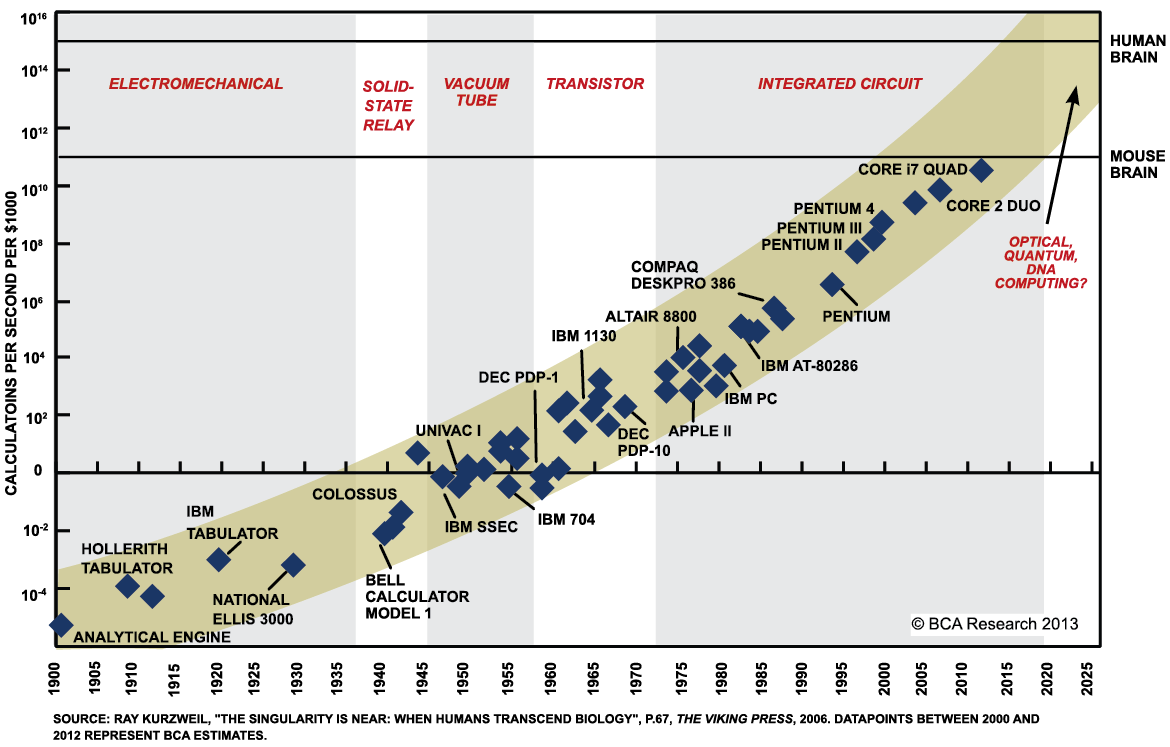
\includegraphics[scale=0.35,center]{MooresLaw}
\caption{Prawo Moora}
\end{figure}

Elementami niezbędnymi do prawidłowego wykreowania wirtualnego środowiska jest zarówno dedykowane oprogramowanie jak i sprzęt konieczny do przekazywania informacji zwrotnych do użytkownika. Rzeczywistość wirtualna aby zostać możliwie najlepiej zinterpretowana przez ludzki mózg musi jak najbardziej przypominać rzeczywistość w której żyjemy na co dzień. Aby sprostać temu zadaniu najczęściej reprezentuje się ją w postaci trójwymiarowych scen. Tylko ten jeden czynnik powoduje, że do poprawnej symulacji niezbędne są nowoczesne, wysokowydajne procesory i karty graficzne będące w stanie przeprowadzić niezbędne obliczenia.

Jak już wspomniano wirtualna rzeczywistość może znajdować zastosowanie także w nauce w szczególności w dziedzinach w których obiekty zainteresowań są zbyt małe aby być widoczne gołym okiem, takie jak cząsteczki chemiczne lub pojedyncze atomy. Istnieje cały szereg programów przeprowadzających np. symulacje oddziaływań międzycząsteczkowych, zwijania białek (ang. protein folding) czy przeprowadzających obliczenia dynamiki molekularnej (ang. molecular dynamics), a także umożliwiających wizualizację tych symulacji. Stosunkowo niewiele jednak jest rozwiązań dedykowanych wirtualnej rzeczywistości, które mogłyby umożliwić interakcję z użytkownikiem za pośrednictwem zmysłu dotyku. 
	
Pracownie Laboratorium Biofizyki na Wydziale Fizyki Uniwersytetu Warszawskiego dysponują sprzętem niezbędnym do realizacji takich zadań. Urządzenie haptyczne Sensable Phantom Omni jest przykładem trójwymiarowego wskaźnika ze zwrotną projekcją momentów sił, którego wykorzystanie otwiera całe spektrum nowych możliwości związanych z realizacją projektów wirtualnej rzeczywiści w biofizyce, biologii molekularnej czy chemii  \cite{vrLecture2011}. 

\chapter*{Cel i zakres pracy}
\addcontentsline{toc}{chapter}{Cel i zakres pracy}

W ramach niniejszej pracy została przedstawiona implementacja aplikacji narzędziowej z pogranicza biofizyki molekularnej i wirtualnej rzeczywistości. Program służący do interaktywnej eksploracji struktur biopolimerów w poszukiwaniu regionów optymalnych ze względu na jakość lokalnego dopasowania strukturalnego pomiędzy wzorcem (ang. template structure) i fragmentami cząsteczki celu (ang. target structure). Jakość znalezionego dopasowania odwzorowuje zwrotna projekcja momentów sił w urządzeniu haptycznym. 
	
Program został zrealizowany w formie wtyczki rozszerzającej możliwości pakietu PyMOL. Do swojego działania wykorzystuje urządzenia i metody wirtualnej rzeczywistości - urządzenie haptyczne Phantom Omni oraz bibliotekę Virtual Reality Peripheral Network - a także bioinformatyczne algorytmy pomiaru jakości dopasowania struktur (RMSD), algorytmy wyszukujące optymalne dopasowanie (ang. alignment) strukturalne oraz algorytmy maksymalizujące stopień dopasowania struktur (algorytm Kabsch'a).

W pracy zostały także przedstawione podstawy teoretyczne leżące u jej podstaw, szczegółowe opisy wykorzystanego urządzenia i metod VR, a także perspektywy dalszego rozwoju i wykorzystania praktycznego opracowanego oprogramowania.

Kod źródłowy stworzonego oprogramowania stanowi integralny załącznik do niniejszej pracy.

\chapter{Podstawy teoretyczne}
W tym rozdziale zaprezentowano podstawową teorię leżącą u podstaw niniejszej pracy. Skupiono się tutaj przede wszystkim na metodach dopasowania (uliniawiania) struktur chemicznych, algorytmach oceny podobieństwa strukturalnego (RMSD), sposobach ich minimalizacji (algorytm Kabsch'a) oraz zagadnieniach związanych z przekształceniami geometrycznymi.

\section{Metody dopasowania struktur chemicznych}
Celem poszukiwania optymalnych metod dopasowania strukturalnego (ang. structural alignment) jest znalezienie homologii pomiędzy cząsteczkami polimerów lub ich fragmentami jedynie na podstawie kształtu i bez znajomości sekwencji. 

Metody dopasowań strukturalnych pierwotnie odnosiły się do cząsteczek polipeptydów i białek jako podstawowych biopolimerów, szybko jednak ich zastosowanie zostało rozszerzone także na kwasy nukleinowe, w szczególności niekodujący RNA gdyż posiada on ważne funkcje biologiczne (np. enzymatyczne) oraz analogiczne do polipeptydów formy drugo- i trzeciorzędowe. 

Z uwagi na znacznie wyższą ewolucyjną trwałość struktury przestrzennej w porównaniu do sekwencji (zarówno aminokwasowej jak i nukleotydowej) poszukiwanie dopasowań strukturalnych często bywa dużo skuteczniejszą metodą znajdowania związków ewolucyjnych pomiędzy organizmami niż klasyczne uliniowienie sekwencji. 

Kluczowym aspektem tych metod jest efektywna ocena ich jakości. Niestety nie ma jednej uniwersalnej miary podobieństwa struktur,  istnieje jednak kilka dobrze opisanych algorytmów służących do szacowania jakości dopasowań strukturalnych. Najczęściej wykorzystywaną do tego celu metryką jest RMSD (ang. root-mean-squared deviation), która zostanie szczegółowo opisana w dalszej części pracy.

Obliczenie dopasowania strukturalnego ponadto implikuje powstanie dopasowania sekwencyjnego pomiędzy przyrównywanymi merami w każdym z łańcuchów. Ocena takiego jednowymiarowego uliniowienia sekwencji również da nam wiedzę o tym jak bliska relacja występuje pomiędzy strukturami.

Z powodu dużej złożoności biopolimerów zostało opracowanych wiele metod upraszczających ich reprezentacje do celów obliczeniowych. Przede wszystkim dąży się do rezygnacji z bezpośredniego rozpatrywania lokalizacji wszystkich atomów pochodzących z każdego meru na rzeczy jedynie tych należących do szkieletu (ang. backbone) cząsteczki (np. $\alpha$-węgle aminokwasów czy pentozy kwasów nukleinowych), z pominięciem lub daleko idącym ograniczeniem roli łańcuchów bocznych.

Metody dopasowania możemy podzielić na globalne, których celem jest porównywanie całych struktur trzeciorzędowych oraz lokalne polegające na poszukiwaniu najlepszego dopasowania fragmentu cząsteczki wzorca (np. struktury drugorzędowej) do wybranego \textit{regionu} (miejsca w obrębie cząsteczki celu) i ewentualna późniejsza ich łączenie do dopasowania globalnego.

\subsection{Globalne dopasowanie struktur} 

Globalne dopasowanie polega na obliczaniu optymalnego nałożenia na siebie (superpozycji) dwóch lub więcej struktur. Jest to iteracyjne podejście, które dąży do minimalizowania odległości pomiędzy atomami (lub wybranymi punktami charakteryzującymi dany mer cząsteczki) w każdym kolejnym kroku poprzez dokonywanie odpowiednich przesunięć i obrotów struktur względem siebie. 

Globalne dopasowanie jest najskuteczniejsze gdy podobieństwo porównywanych struktur jest ma tyle wysokie aby obliczenia dążyły do optymalnego globalnie rezultatu. Jest to często stosowana metoda służąca do porównywania różnych konformacji tego samego polimeru, na przykład do oceny jakości algorytmów przewidujących strukturę białek lub porównywanie struktur analogicznych białek pochodzących z różnych organizmów. 

\begin{figure}[H]
\centering
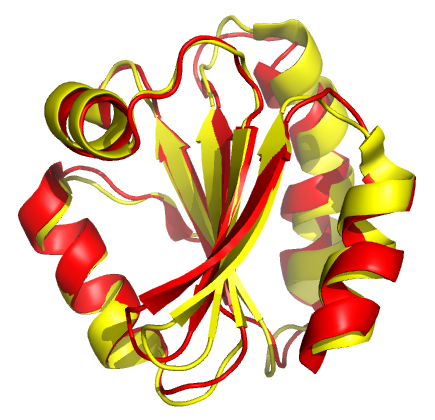
\includegraphics[scale=0.7]{global_superposition}
\caption{Superpozycja dwóch struktur tioredoksyny (białko o długości 105 aminokwasów) ludzkiej (kolor czerwony) i pochodzącej z muszki owocowej \textit{Drosophila melanogaster} (kolor żółty), RMSD=1.244\AA }
\end{figure}

\subsection{Lokalne dopasowanie struktur} 
Jak już wspomniano, lokalne dopasowanie polega na przeszukiwaniu części lub całości cząsteczki celu (ang. target) w poszukiwaniu takich regionów, które \textit{są podobne} do wybranych struktur zwanych wzorcami (ang. template). Wzorcami mogą być na przykład struktury drugorzędowe, miejsca wiążące lub inne dowolnie wybrane fragmenty cząsteczek. Z grupy odpowiednio wybranych lokalnych dopasowań próbuje się budować uliniowienie globalne.
\\
\\
\textbf{TODO: skąd dokładnie pochodzą dane wejściowe (plik mapujący) do tego programu? czy jego podstawą są lokalne deskryptory struktury? }
\\
\textbf{UWAGA: uzupełnić i poprawić błędy w dalszej części podrozdziału}
\\
\\
Spośród wielu opracowanych metod realizacji lokalnego dopasowania, warto wspomnieć przede wszystkim o metodzie opartej o \textit{lokalne deskryptory struktury} \cite{daniluk11}. Stanowi ona (?? czy napewno tak jest??) podstawę implementacji oprogramowania dostarczającego dane wejściowe do programu będącego przedmiotem niniejszej pracy. 

\textit{Lokalne deskryptory struktury białek} stanowią pewną abstrakcję opisującą otoczenie każdego aminokwasu... 

\textbf{<czy tą metodę wykorzystuje się jedynie do białek? czy można do RNA? >}

Wynikiem przeprowadzonych operacji lokalnego dopasowania jest indeks miejsc do których wzorzec jest \textit{podobny} wraz z ich miarą dopasowania. Należy pamiętać, że jeden wzorzec może być podobny do wielu regionów w obrębie tej samej cząsteczki celu, przez co może występować w wielu miejscach w ramach indeksu mapującego.

Rezultatem działania ww. programu jest plik mapujący, który zawiera informacje o wszystkich miejscach dla których został przekroczony zadany próg podobieństwa do struktury wzorca \textbf{CZY napewno tam jest jakiś próg??}. Innymi słowy uzyskujemy kompletną mapę cząsteczki celu z wyróżnionymi regionami, których superpozycja ze strukturą wzorca daje stopień podobieństwa nie gorszy niż zadany próg.


\section{RMSD}
Efektywna ocena podobieństwa struktur chemicznych jest jednym z kluczowych elementów procesu dopasowania strukturalnego. W bioinformatyce istnieje kilka sposobów oszacowania tej wartości: obok GDT (ang. global distance test) i TM-score (ang. template modeling score) \cite{zhangSkolnick2005} najpopularniejsza i stosunkowo prosta w zastosowaniu jest miara odchylenia średniokwadratowego - RMSD (ang. root-mean-squared deviation) \cite{kufarevaAbagyan2012}. 

Ocena podobieństwa metodą RMSD polega na obliczeniu średniokwadratowej odległości pomiędzy współrzędnymi odpowiadających sobie atomów (lub innych punktów charakterystycznych) zawartych w strukturze wzorca (ang. template) i cząsteczce celu (ang. target). W tym przypadku jednostką najczęściej jest \AA (angstrom). Dwie struktury są tym bardziej do siebie podobne im bliższa zeru jest wartość RMSD.

$$
\begin{array}{lr}
RMSD(p,q) = \sqrt{\frac{1}{N}\sum_{i=1}^{N}||p_i-q_i||^{2}} = \\
\\
= \sqrt{\frac{1}{N}\sum_{i=1}^{N}((p_{ix}-q_{ix})^{2}+(p_{iy}-q_{iy})^{2}+(p_{iz}-q_{iz})^{2})}
\end{array}
$$
\\
gdzie:
\\
$p$ - wektor punktów struktury wzorca
\\
$q$ - wektor punktów wybranego regionu w strukturze celu
\\
$N$ - długość wektorów współrzędnych $p$ i $q$
\\
\\
O ile same obliczenia są trywialne, to dobór danych wejściowych do algorytmu RMSD może stanowić poważne wyzwanie. 

W tym przypadku dane pochodzą z zewnętrznej aplikacji, która wykonuje procedurę dopasowania (uliniowienia) struktur wzorca i celu oraz odnajduje takie regiony, których miara podobieństwa nie przekracza zadanego progu (ang. threshold). Wynikiem takiej procedury są dane mapujące (ang. mapping file) zawierające informację o lokalizacji \textit{regionów podobnych} do struktury wzorca w cząsteczce celu. Takimi regionami mogą być dowolne struktury drugorzędowe (w szczególności alfa-helisy czy beta-harmonijki) lub trzeciorzędowe.

\begin{figure}[H]
\centering
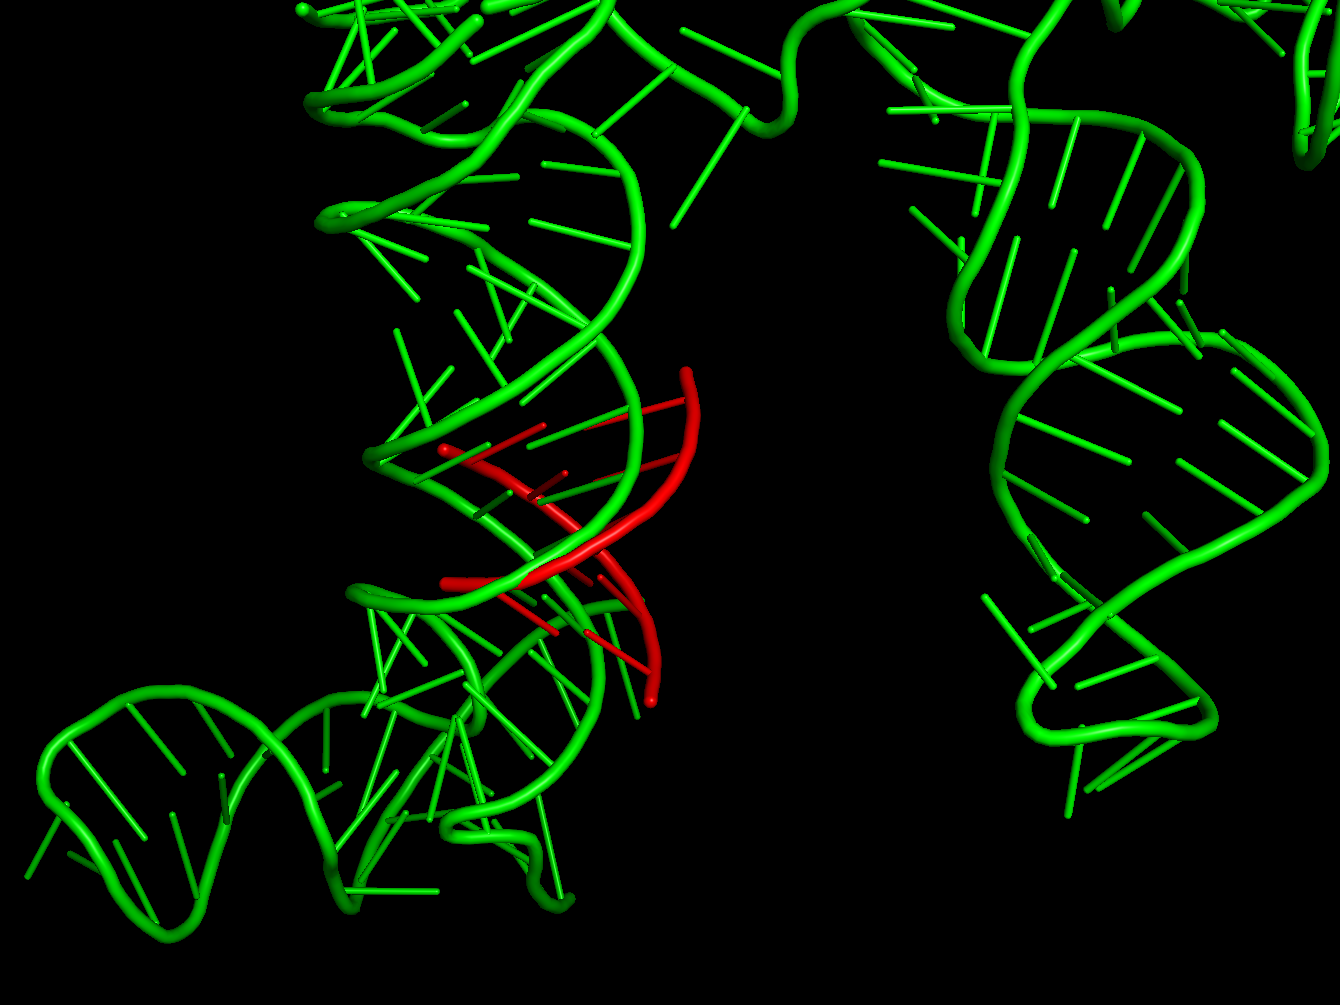
\includegraphics[scale=0.2]{rmsd3}
\caption{Przykładowe dopasowanie struktury wzorca (czerwona) do podobnego regionu struktury celu (zielona), RMSD=3.985}
\end{figure}


\begin{figure}[H]
\centering
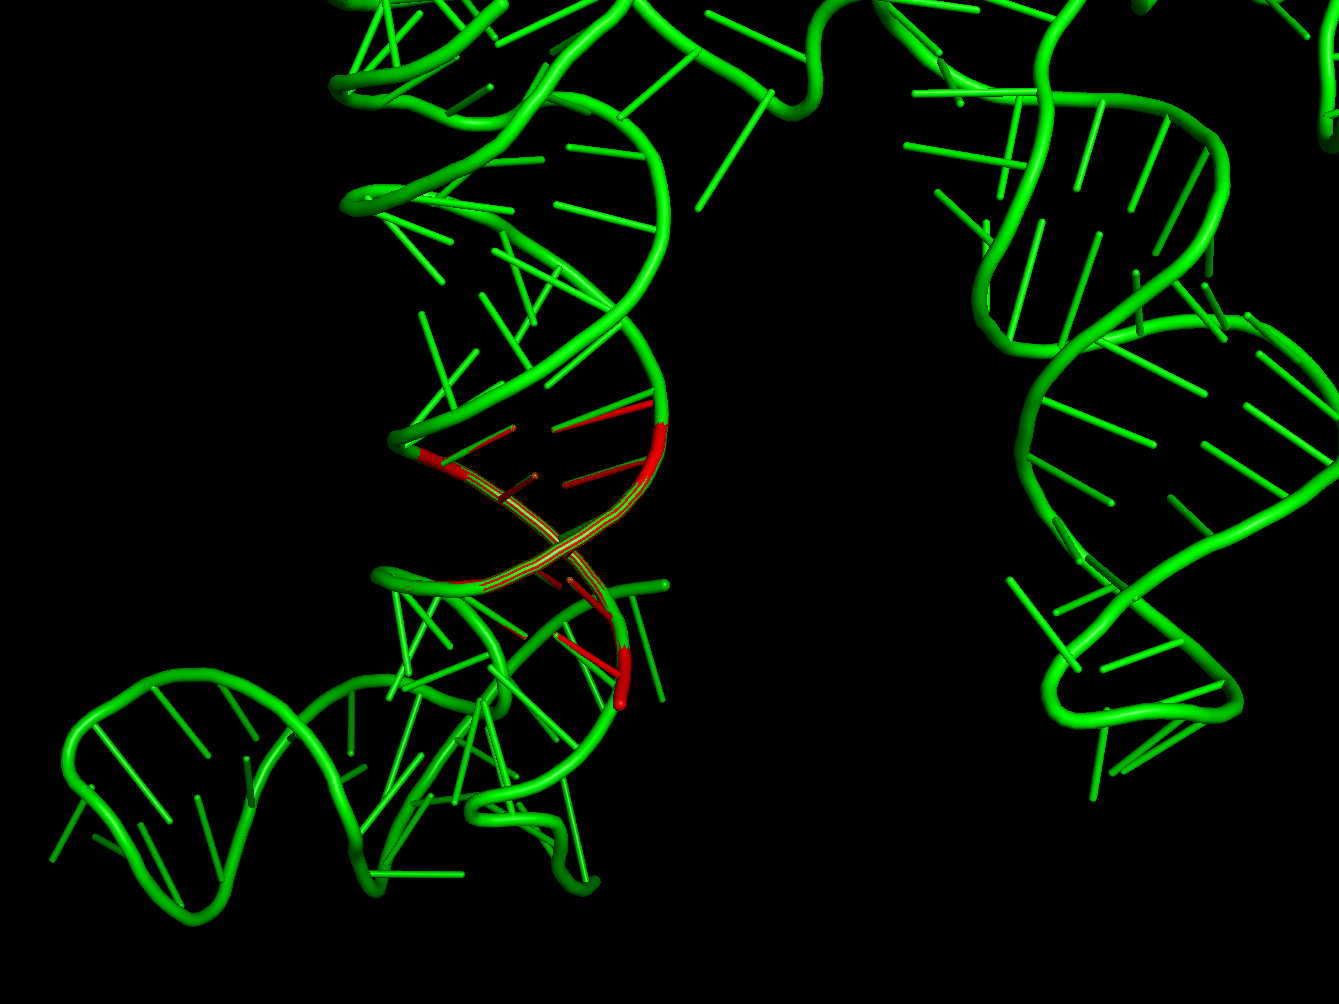
\includegraphics[scale=0.2]{rmsd0}
\caption{Przykładowe dopasowanie struktury wzorca (czerwona) do podobnego regionu struktury celu (zielona), RMSD=0}
\end{figure}

\section{Algorytm Kabsch'a}
RMSD jest jedną podstawowych miar podobieństwa strukturalnego wykorzystywanych w bioinformatyce. Jednym ze znanych sposobów minimalizacji jej wartości (maksymalizacji dopasowania) jest optymalna translacja i rotacja struktury wzorca nad wybranym regionem struktury celu w taki sposób aby obie struktury zostały jak najlepiej na siebie nałożone. Istnieje kilka metod wyznaczania optymalnych transformacji, jedną z popularniejszych opisał opisał w 1976 roku w swojej pracy Wolfgang Kabsch \cite{kabsch1976} i \cite{kabsch1978}.

Algorytm startuje z dwoma wektorami współrzędnych $p$ i $q$ o długości $N$:
$$
p=
\begin{pmatrix}
 x_{p1} & y_{p1} & z_{p1} \\
 x_{p2} & y_{p2} & z_{p2} \\
 \vdots & \vdots & \vdots \\
 x_{pN} & y_{pN} & z_{pN}
\end{pmatrix}
$$
$$
q= 
\begin{pmatrix}
 x_{q1} & y_{q1} & z_{q1} \\
 x_{q2} & y_{q2} & z_{q2} \\
 \vdots & \vdots & \vdots \\
 x_{qN} & y_{qN} & z_{qN}
\end{pmatrix}
$$
\\
gdzie:
\\
$p$ wektor punktów struktury wzorcowej
\\
$q$ wektor punktów wybranego regionu struktury celu
\\
\\
Algorytm Kabsch'a składa się z 3 kroków (http://cnx.org/contents/HV-RsdwL@23/Molecular-Distance-Measures):
\begin{enumerate}
\item \textbf{Translacja} \\
W pierwszym kroku należy dokonać obliczenia centroidów ($Cp$ i $Cq$) obu struktur i dokonać przesunięcia struktury wzorca o wektor $\vec{T}$ rozpięty pomiędzy tymi punktami tak, aby nałożyły się one na siebie. Do obliczenia centroidu można posłużyć się wzorem na średnią arytmetyczną wartości poszczególnych współrzędnych: 
$$Cp = (Cp_x, Cp_y, Cp_z)$$
gdzie:
$$Cp_x = \frac{1}{N}\sum_{i=1}^{N}{x_{pi}}$$
$$Cp_y = \frac{1}{N}\sum_{i=1}^{N}{y_{pi}}$$
$$Cp_z = \frac{1}{N}\sum_{i=1}^{N}{z_{pi}}$$
oraz
$$Cq = (Cq_x, Cq_y, Cq_z)$$
gdzie:
$$Cq_x = \frac{1}{N}\sum_{i=1}^{N}{x_{qi}}$$
$$Cq_y = \frac{1}{N}\sum_{i=1}^{N}{y_{qi}}$$
$$Cq_z = \frac{1}{N}\sum_{i=1}^{N}{z_{qi}}$$
zatem wektor translacji $\vec{T}$ taki, że:
$$ \vec{T} = |Cp-Cq| =(|Cp_x-Cq_x|,|Cp_y-Cq_y|,|Cp_z-Cq_z|)$$
możemy użyć do wykonania przesunięcia wszystkich punktów w $p$ i $q$:
$$p'=p+\vec{T}$$
\item \textbf{Macierz kowariancji} \\
Po wykonanym przesunięciu należy obliczyć zależność liniową pomiędzy współrzędnymi wektorów $p'$ i $q$. Poprawne wyliczenie macierzy kowariancji $A$ będzie także stanowiło podstawę do ustalenia optymalnej macierzy rotacji (w kolejnym kroku):
$$ 
A=cov(p',q)
$$
lub równoważnie w zapisie macierzowym:
$$
 A = p'q^T
$$

\item \textbf{Optymalna macierz rotacji} \\
Optymalna macierz rotacji powstaje z \textit{dekompozycji według wartości szczególnych} macierzy $A$. SVD (ang. singular value decomposition) to taki rozkład zadanej macierzy na trzy specyficzne macierze $U$, $\Sigma$ oraz $V$, że zachodzi zależność:
$$
A=U \Sigma V^T
$$
gdzie:
\\
$U$ i $V$ to macierze ortogonalne (takie, że $U^{-1}=U^{T}$ oraz $V^{-1}=V^{T}$)
\\
$\Sigma$ macierz diagonalna (taka, że na przekątnej mamy nieujemne liczby rzeczywiste, będące \textit{wartościami szczególnymi} macierzy A)
\\
\\
Sprawdzając znak wartość wyznacznika:
$$
s=sign(det(VW^T))
$$
upewniamy się, że operujemy w ramach prawoskrętnego układu współrzędnych. Ostatecznie uzyskujemy optymalną macierz rotacji $R$:

$$
R=V
\begin{pmatrix}
 1 & 0 & 0 \\
 0 & 1 & 0 \\
 0 & 0 & s
\end{pmatrix}
U^T
$$

\end{enumerate}

\section{Przekształcenia geometryczne i ich reprezentacje}
Przekształcenia geometryczne w przestrzeni trójwymiarowej są istotnymi operacjami używanymi w niniejszej pracy \cite{vanDam2000}. Zaliczamy do nich przede wszystkim skalowanie, translacje i rotacje. Wszystkie te operacje można praktycznie zrealizować na kilka sposobów. Ze względu na to, że operują na milionach punktów w przestrzeni trójwymiarowej (pikseli), \textit{optymalne metody numeryczne} które je realizują są niezmiernie ważne i muszą w maksymalnym stopniu wykorzystywać możliwości oferowane przez komputerowe jednostki obliczeniowe i procesory graficzne. 

Współpraca bibliotek programistycznych pochodzących od różnych dostawców może wymagać wielu przekształceń pomiędzy różnymi formatami opisu transformacji. Szczególną uwagę należy zwrócić na konwersję orientacji wskaźnika urządzenia haptycznego z kwaternionów (postaci dostarczanej przez bibliotekę VRPN) na \textit{oś i kąt obrotu} (akceptowany przez PyMOL) i odwrotnie.

Z uwagi na konieczność dostosowania transformacji do wykonywania na współczesnych komputerach niezbędne było opracowanie efektywnych obliczeniowo metod numerycznych i reprezentacji tych operacji. Bezpośrednia ich implementacja byłaby dość kłopotliwa gdyż nie dość, że każda transformacja musiałaby zostać wykonana oddzielnie (sekwencyjnie), to przede wszystkim nie byłoby to optymalne obliczeniowo rozwiązanie. Do tego celu wybrano ujednolicone narzędzia rozwiązujące powyższe problemy: \textit{elementarne macierze transformacji} i \textit{współrzędne jednorodne}.

\textit{Elementarne macierze transformacji} stanowią łatwe narzędzie matematyczne do operowania przekształceniami geometrycznymi. Każda z transformacji może zostać opisana jako prosta operacja macierzowa (dodawanie albo mnożenie) modyfikująca zbiór punktów w przestrzeni.

Często pojawia się sytuacja w której kilka przekształceń geometrycznych chcemy wykonać jednocześnie. Można sobie wyobrazić taki przypadek w którym obiekt chcemy jednocześnie przesunąć i dokonać jego obrotu. Niestety stosowanie ,,surowych'' elementarnych macierzy transformacji uniemożliwia rozwiązanie tej kwestii, dopiero \textit{współrzędne jednorodne} pozwoliły w pełni wyeliminować ten problem.

\textit{Współrzędne jednorodne} są sposobem reprezentacji punktów przestrzeni $n$-wymiarowej za pomocą układu $n+1$ współrzędnych. Zostały one wprowadzone przez niemieckiego matematyka Augusta Möbiusa w 1827 roku i opisane w jego pracy \textit{Der barycentrische Calcul}. 

Współrzędne jednorodne to narzędzie matematyczne stanowiące pewne udoskonalenie elementarnych macierzy transformacji. Umożliwiają wykonywanie wielu przekształceń jednocześnie i za pomocą jednej operacji macierzowej - mnożenia. Współrzędne jednorodne dają możliwość skumulowania wszystkich transformacji jakie chcemy wykonać na strukturze przestrzennej w jednej odpowiednio zbudowanej macierzy. W dzisiejszych czasach zostały one docenione w wielu dziedzinach nie tylko bezpośrednio związanych z grafiką komputerową ale także w robotyce czy biofizyce.

Poniżej szczegółowo opisane zostały wykorzystane w pracy transformacje: skalowanie, translacja oraz rotacja. Dla każdej z nich podane zostały ich reprezentacje za pomocą elementarnych macierzy transformacji oraz współrzędnych jednorodnych. Dodatkowo dla rotacji została przedstawiona reprezentacja w kwaternionach.

\subsection{Skalowanie}
Skalowanie to operacja polegająca na mnożeniu współrzędnych obiektu określonego w przestrzeni trójwymiarowej przez współczynniki skalowania. Współczynniki skalowania są dodatnią liczbą rzeczywistą $S$ albo dodatnio określonym wektorem liczb rzeczywistych $\vec{S}$. 

W ogólności możemy skalować wszystkie składowe wektora współrzędnych niezależnie przez stosowanie wektora o różnych współczynnikach $\vec{S}$, jednak dla potrzeb niniejszej pracy ograniczymy się do mnożenia wektora współrzędnych wyłącznie przez skalar $S$.

Geometryczna intuicja stojąca za operacją skalowania polega na takim przekształceniu współrzędnych danego obiektu, że w zależności od wartości współczynnika skalującego może on zostać: 
\\
- niezmieniony, gdy $S=1$
\\
- pomniejszony proporcjonalnie do $S$, gdy $0<S<1$
\\
- powiekszony proporcjonalnie do $S$, gdy $S>1$
\\
\\
Współrzędne dowolnego punktu $P=(x,y,z)$ po operacji skalowania o współczynnik $S$ są równe $P'=(x',y',z')$, gdzie:

$$
\begin{array}{lr}
x'=x*S \\
y'=y*S \\
z'=z*S
\end{array}
$$

Reprezentacja skalowania za pomocą elementarnych macierzy transformacji polega na stworzeniu takiej macierzy $\hat{S}$, że wartość współczynnika $S$ zostanie wpisane do niej w następujący sposób:
$$
\hat{S}
=
\begin{bmatrix}
S & 0 & 0 \\
0 & S & 0 \\
0 & 0 & S
\end{bmatrix}
$$
zatem w zapisie macierzowym otrzymujemy:
$$
\vec{P'}=\hat{S}*\vec{P}
$$

$$
\vec{P'}
=
\begin{bmatrix}
S & 0 & 0 \\
0 & S & 0 \\
0 & 0 & S
\end{bmatrix}
*
\begin{bmatrix} 
x \\ 
y \\ 
z 
\end{bmatrix} 
=
\begin{bmatrix} 
x*S \\ 
y*S \\ 
z*S 
\end{bmatrix}
$$
\\
Aby przedstawić operację skalowania we współrzędnych jednorodnych należy stworzyć nową macierz $\bar{S}$ o rozmiarze o 1 większym niż macierz elementarna $\hat{S}$ oraz nowy wektor $\dot{\vec{P}}$ o długości o 1 większej niż $\vec{P}$, taki że:
$$
\bar{S} 
= 
\begin{bmatrix}
S & 0 & 0 & 0 \\
0 & S & 0 & 0 \\
0 & 0 & S & 0 \\
0 & 0 & 0 & 1
\end{bmatrix}
,  
\dot{\vec{P}}
=
\begin{bmatrix} 
x \\ 
y \\ 
z \\
1
\end{bmatrix} 
$$
zatem:
$$
\dot{\vec{P'}}=\bar{S}*\dot{\vec{P}}
$$
$$
\dot{\vec{P'}} = 
\begin{bmatrix}
S & 0 & 0 & 0 \\
0 & S & 0 & 0 \\
0 & 0 & S & 0 \\
0 & 0 & 0 & 1
\end{bmatrix}
*
\begin{bmatrix} 
x \\ 
y \\ 
z \\
1
\end{bmatrix} 
=
\begin{bmatrix} 
x*S \\ 
y*S \\ 
z*S \\
1
\end{bmatrix}
$$

\subsection{Translacje}
Translacje to kolejna elementarna operacja przekształcenia geometrycznego. Translacją nazywamy takie przekształcenie, które przesuwa każdy punkt zbioru określony w przestrzeni o dowolny wektor $\vec{T}$. W odróżnieniu od skalowania, w przypadku przesunięć w przestrzeni do wektora współrzędnych dodajemy wektor współczynników (liczb rzeczywistych) przesunięcia $\vec{T}$. W niniejszej pracy operacja przesunięcia wykonywana jest przy każdej zmianie położenia wskaźnika urządzenia haptycznego oraz podczas wykonywania operacji nałożenia i dopasowania struktur. 

Dla zadanego punktu $P=(x,y,z)$ efektem operacji przesunięcia o wektor $\vec{T}=[t_x, t_y, t_z]^T$ są współrzędne $\vec{P'}=(x',y',z')$:

$$
\begin{array}{lr}
x'=x+t_x \\
y'=y+t_y \\
z'=z+t_z
\end{array}
$$
Z powyższego jasno wynika, że translacje można reprezentować jako operację sumy dwóch wektorów:
$$
\vec{P'}=\vec{P}+\vec{T}
$$
$$
\vec{P'}
=
\begin{bmatrix}
x \\
y \\
z
\end{bmatrix}
+
\begin{bmatrix}
t_x \\
t_y \\
t_z 
\end{bmatrix}
=
\begin{bmatrix}
x+t_x \\
y+t_y \\
z+t_z 
\end{bmatrix}
$$

Translacje można przedstawić także za pomocą współrzędnych jednorodnych. Wymaga to stworzenia macierzy $\bar{T}$ oraz wektora $\dot{\vec{P}}$, takich że:
$$
\bar{T}
=
\begin{bmatrix}
1 & 0 & 0 & t_x \\
0 & 1 & 0 & t_y \\
0 & 0 & 1 & t_z \\
0 & 0 & 0 & 1
\end{bmatrix}
,
\dot{\vec{P}}
=
\begin{bmatrix}
x \\
y \\
z \\
1
\end{bmatrix}
$$
zatem:
$$
\vec{P'}=\bar{T}*\dot{\vec{P}}
$$
$$
\vec{P'}=
\begin{bmatrix}
1 & 0 & 0 & t_x \\
0 & 1 & 0 & t_y \\
0 & 0 & 1 & t_z \\
0 & 0 & 0 & 1
\end{bmatrix}
*
\begin{bmatrix}
x \\
y \\
z \\
1
\end{bmatrix}
=
\begin{bmatrix}
x+t_x \\
y+t_y \\
z+t_z \\
1
\end{bmatrix}
$$
\subsection{Rotacje i kwaterniony}
Trzecią elementarną transformacją jest rotacja, która w odróżnieniu od skalowania czy translacji jest operacją bardziej złożoną. Należy zwrócić uwagę, że kolejność wykonywania rotacji ma znaczenie ($R_xR_y\neq R_yR_x$), po drugie samych reprezentacji rotacji jest co najmniej kilka. Najpopularniejszym z nich są obroty o zadany kąt wokół jednej z osi układu współrzędnych lub arbitralnej osi obrotu.

Współrzędne punktu $P'=(x',y',z')$ będącego wynikiem rotacji punktu $P=(x,y,z)$ wokół poszczególnych osi ($OX$, $OY$, $OZ$) układu współrzędnych o zadany kąt (odpowiednio $\alpha$, $\beta$ i $\gamma$) wyrażają się następująco:
\\
\\
rotacja $P$ wokół osi $OX$:
$$
\begin{array}{lr}
x'=x \\
y'=ycos(\alpha)-zsin(\alpha) \\
z'=ysin(\alpha)+zcos(\alpha)
\end{array}
$$
\\
rotacja $P$ wokół osi $OY$:
$$
\begin{array}{lr}
x'=zsin(\beta)+xcos(\beta) \\
y'=y \\
z'=xcos(\beta)-xcos(\beta)
\end{array}
$$
\\
rotacja $P$ wokół osi $OZ$:
$$
\begin{array}{lr}
x'=xcos(\gamma)-ysin(\gamma) \\
y'=xsin(\gamma)+ycos(\gamma) \\
z'=z
\end{array}
$$
Elementarne macierze przekształceń w tym przypadku wyglądają następująco:
$$
\hat{Rx}(\alpha)
=
\begin{bmatrix}
1 & 0 & 0 \\
0 & cos(\alpha) & -sin(\alpha) \\
0 & sin(\alpha) & cos(\alpha)
\end{bmatrix}
$$
$$
\hat{Ry}(\beta)
=
\begin{bmatrix}
cos(\beta) & 0 & sin(\beta) \\
0 & 1 & 0 \\
-sin(\beta) & 0 & cos(\beta) \\
\end{bmatrix}
$$
$$
\hat{Rz}(\gamma)
=
\begin{bmatrix}
cos(\gamma) & -sin(\gamma) & 0 \\
sin(\gamma) & cos(\gamma) & 0 \\
0 & 0 & 1
\end{bmatrix}
$$
gdzie:
\\
$\hat{Rx}(\alpha)$ obrót wokół osi $OX$ o kąt $\alpha$
\\
$\hat{Ry}(\beta)$ obrót wokół osi $OY$ o kąt $\beta$
\\
$\hat{Rz}(\gamma)$ obrót wokół osi $OZ$ o kąt $\gamma$
\\
\\
Jak wszystkie inne transformacje, rotacje równiez można przedstawić we współrzędnych jednorodnych. Odpowiednie macierze mają wówczas następującą postać:
$$
\bar{Rx}(\alpha) = 
\begin{bmatrix}
1 & 0 & 0 & 0 \\
0 & cos(\alpha) & -sin(\alpha) & 0 \\
0 & sin(\alpha) & cos(\alpha) & 0 \\
0 & 0 & 0 & 1
\end{bmatrix}
$$
$$
\bar{Ry}(\beta) = 
\begin{bmatrix}
cos(\beta) & 0 & sin(\beta) & 0 \\
0 & 1 & 0 & 0 \\
-sin(\beta) & 0 & cos(\beta) & 0 \\
0 & 0 & 0 & 1
\end{bmatrix}
$$
$$
\bar{Rz}(\gamma) = 
\begin{bmatrix}
cos(\gamma) & -sin(\gamma) & 0 & 0 \\
sin(\gamma) & cos(\gamma) & 0 & 0 \\
0 & 0 & 1 & 0 \\
0 & 0 & 0 & 1
\end{bmatrix}
$$

Rotacje reprezentowane przez współrzędne jednorodne można dowolnie ze sobą łączyć poprzez mnożenie odpowiednich macierzy, należy jednak mieć na uwadze fakt (jak już wcześniej wspomniano), że rotacje nie są przemienne - kolejność wykonywanych operacji ma znaczenie.
\\
\\
Rotacje posiadają jeszcze jedną być może najważniejszą z punktu widzenia programisty reprezentację: \textit{kwaterniony} \cite{magarshak1992}. Są one strukturą algebraiczną stanowiącą rozszerzenie liczb zespolonych. Kwaterniony zostały wprowadzone przez Williama Hamiltona \cite{hamilton1843}, który poszukiwał wygodnego sposobu opisu mechaniki w przestrzeni trójwymiarowej. 

Kwaternion $q$ to taka czwórka liczb rzeczywistych $x$, $y$, $z$ i $w$ spełniająca równanie:
$$
q=w+xi+yj+zk
$$
gdzie:
\\
$i$, $j$, $k$ - współczynniki urojone takie, że $i^2=j^2=k^2=ijk=-1$
\\
$w$ - część skalarna kwaterniona
\\
$x$, $y$, $z$ - część wektorowa kwaterniona
\\
\\
Kwaterniony mogą stanowić alternatywną wobec współrzędnych jednorodnych lub macierzy transformacji formę opisu rotacji. Możemy z powodzeniem przeprowadzać konwersję pomiędzy różnymi reprezentacjami rotacji.

Dzięki kwaternionom z można przedstawić rotację wokół arbitralnie wybranej osi (wektora) obrotu. Załóżmy, że chcemy stworzyć kwaternion $q$ reprezentujący obrót o kąt $\alpha$ wokół wektora $\vec{v}=[v_x,v_y,v_z]$. Kwaternion taki tworzymy w następujący sposób

$$
\begin{array}{lr}
w=cos(\alpha/2) \\
x=v_x sin(\alpha/2) \\
y=v_y sin(\alpha/2) \\
z=v_z sin(\alpha/2) 
\end{array}
$$

wówczas:
$$
q=cos(\alpha/2)+v_xsin(\alpha/2)i+v_ysin(\alpha/2)j+v_zsin(\alpha/2)k
$$

Kwaterniony mogą reprezentować nie tylko rotację (obrót bryły) ale także orientację (stan bryły). Biblioteka VRPN (wykorzystana w niniejszej pracy) wydaje informację o bieżącej orientacji wskaźnika, natomiast pakiet PyMOL akceptuje jedynie \textit{zmiany orientacji} (rotacje). 

Prawidłowe wykonanie rotacji z dwóch kolejnych kwaternionów $q_n$ i $q_{n+1}$ niosących informację o orientacji polega na zastosowaniu odwrotnego kwaterniona $q_n^{-1}$ (powracającego strukturę do orientacji początkowej, \textit{zerowej}) i dopiero później kwaterniona $q_{n+1}$. Taki ciąg operacji należy wykonywać cyklicznie w miarę odbierania kolejnych informacji o orientacji wskaźnika. Kwaternion odwrotny jest zdefiniowany następująco:

$$
q^{-1}=\frac{w-xi-yj-zk}{w^2+x^2+y^2+z^2}
$$


\section{Pole siłowe}
Biblioteka VRPN dostarcza kilku metod sterowania zwrotną projekcją sił (szerszy opis w dalszej części). W tej pracy wykorzystano tzw. metodę pola siłowego (ang. force field), która podobnie jak w pozostałych metodach (np. powierzchnia lub bryła) realizowana jest przez lokalną aproksymację. Jej wywołanie polega na dostarczeniu funkcji trzech parametrów: punktu zaczepienia (ang. origin), wektora siły oraz macierzy Jacobiego.

Punktem zaczepienia wektora siły jest w tym przypadku środek geometryczny wzorcowej struktury chemicznej obliczany jako średnia arytmetyczna wartości poszczególnych współrzędnych.

Wektor siły to wektor wskazujący kierunek i zwrot siły działającej na wskaźnik. W tym przypadku jest on rozpięty pomiędzy środkami geometrycznymi struktury wzorcowej, a najbliższym \textit{podobnym} regionem - wyznaczonym przez algorytm dopasowania strukturalnego. Zwrot siły jest skierowany w stronę owego regionu. Do dalszych rozważań możemy traktować wektor $\vec{F}$ jako iloczyn wektora jednostkowego (wersora) $\dot{F}$ oraz skalarnej wartości siły force:
$$
\vec{F}=\dot{F}*force=[\vec{F_x}*force,\vec{F_y}*force,\vec{F_z}*force]
$$

Macierz Jacobiego $J_{\vec{F}}$ jest macierzą zbudowaną z pochodnych cząstkowych pierwszego rzędu funkcji definiującej pole siłowe. Tutaj różniczkowaniu poddawane są poszczególne składowe wektora siły $\vec{F}$:

$$
J_{\vec{F}}=
\begin{bmatrix}
\frac{\delta \vec{F_x}}{\delta x} & \frac{\delta \vec{F_y}}{\delta x} & \frac{\delta \vec{F_z}}{\delta x} \\
\frac{\delta \vec{F_x}}{\delta y} & \frac{\delta \vec{F_y}}{\delta y} & \frac{\delta \vec{F_z}}{\delta y} \\
\frac{\delta \vec{F_x}}{\delta z} & \frac{\delta \vec{F_y}}{\delta z} & \frac{\delta \vec{F_z}}{\delta z}
\end{bmatrix}
=
\begin{bmatrix}
force & 0 & 0 \\
0 & force & 0 \\
0 & 0 & force
\end{bmatrix}
$$
	
\chapter{Urządzenie haptyczne Sensable Phantom Omni}
Nadrzędnym celem wirtualnej rzeczywistości jest możliwie wierne odtworzenie świata rzeczywistego lub fikcyjnego w formie programu komputerowego czy multimedialnej prezentacji. Ponadto metody i narzędzia wirtualnej rzeczywistości umozliwiają użytkownikowi wchodzenie w czynna interakcję z tak wykreowanymi scenami. Obecny stan rozwoju techniki pozwala na tworzenie wydajnych urządzeń klasy HCI (ang. human computer interface) będących interfejsami pomiędzy światem realnym a wirtualnym. Przykładem takiego urządzenia jest Phantom Omni, opracowane przez firmę SensAble (obecnie Geomagic). 

\begin{figure}[H]
\centering
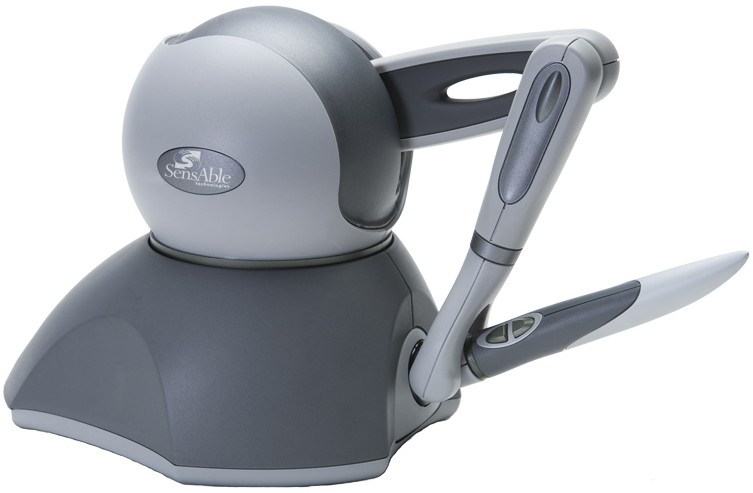
\includegraphics[scale=0.5,center]{Sensable_Phantom_Omni}
\caption{Urządzenie haptyczne SensAble Phantom Omni}
\end{figure}

Niniejsza praca w znacznym stopniu opiera się na wykorzystaniu tych urządzeń do odzworowywania rzeczywistych ruchów ręki użytkownika w świecie wirtualnym. Pracownie Zakładu Biofizyki Wydziału Fizyki Uniwersytetu Warszawskiego są wyposażone w tego typu urządzenia, zostały one udostępnione autorowi celem realizacji niniejszej pracy.

\section{Opis urządzenia}
Urządzenie haptyczne (ang. haptic device) Sensable Phantom Omni jest trójwymiarowym wskaźnikiem o 6 stopniach swobody wskazywania pozycji i orientacji. Urządzenie ma także możliwość programowego sterowania zwrotną projekcją (ang. force feedback) momentów sił w trzech stopniach swobody (sterowanie pozycją wskaźnika). Ponadto w urządzeniach dostępne są dwa przyciski monostabilne do dowolnego wykorzystania.

Phantom Omni jest urządzeniem znajdującym zastosowanie w różnego rodzaju aplikacjach działających na styku świata wirtualnego z rzeczywistym. Umożliwia ono użytkownikowi wchodzenie w interakcję z cyfrowym światem za pomocą \textit{zmysłu dotyku}. Dzięki dostarczonym przez producenta sterownikom i bogatemu zestawowi bibliotek i narzędzi programistycznych OpenHaptics możliwe jest tworzenie oprogramowania w pełni wykorzystującego możliwości oferowane przez urządzenie.

Specyfikację techniczną urządzenia prezentuje poniższa tabela \cite{geomagicTouchBrochure}:

\begin{center}
	\begin{tabular}{|l|p{4cm}|}
		\hline Wymiary pola roboczego & szerkość: 160 mm $\newline$ głębokość 70 mm $\newline$ wysokość 120 mm \\
		\hline Rozdzielczość & 450 dpi ($\sim$0.055 mm) \\
		\hline Maksymalny moment obrotowy & 3.3 Nm \\
		\hline Sztywność & oś X: 1.26 N/mm $\newline$ oś Y: 2.31 N/mm $\newline$ oś Z: 1.02 N/mm \\
 		\hline Dane o pozycji i orientacji & osi X, Y i Z $\newline$ kąty $\alpha$, $\beta$ i $\gamma$ $\newline$ (6 stopni swobody)\\
		\hline Zwrotna projekcja sił & osi X, Y i Z $\newline$ (3 stopnie swobody) \\
		\hline Interfejs & IEEE-1394a $\newline$ Ethernet \\
		\hline
	\end{tabular}
\end{center}	
	
\section{Wymagania sprzętowe}

	Urządzenia Sensable Phantom Omni w które wyposażone są Pracownie Biofizyki FUW posiadają dwa rodzaje interfejsów: Ethernet oraz FireWire (IEEE-1394a). 

Interfejs Ethernet jest powszechnie spotykany w większości komputerów i systemy operacyjne bezproblemowo radzą sobie z jego obsługą. Użycie urządzenia Phantom Omni z interfejsem sieciowym wiąże się jednak z instalacją dedykowanych sterowników oraz pakietu OpenHaptics v3.0, które jak podaje producent są wspierają jedynie systemy do Windows 8 włącznie, co uniemożliwia korzystanie z nich na nowszych platformach.

FireWire jest standardem łącza szeregowego opracowanym w 1995 roku, który umożliwia szybką transmisję danych. Został on zaprojektowany przede wszystkim do szybkiego przesyłania danych o dużym rozmiarze, zatem jest często wykorzystywany przez producentów sprzętu multimedialnego. Jednak w związku z systematycznym wycofywaniem się (od 2011 roku) producentów sprzętu i oprogramowania ze wspierania interfejsu FireWire, korzystanie z urządzeń w niego wyposażonych rodzi wiele problemów. Użytkownik jest zmuszony do poszukiwania dedykowanych (spełniających specyficzne wymagania producenta) kart rozszerzeń do stacji roboczych mających obsługiwać urządzenia - na dodatek firma SenseAble zaleca korzystanie wyłącznie z kontrolerów IEEE-1394a opartych o chipset firmy NEC lub VIA co może dodatkowo utrudnić proces wdrażania urządzeń przy stanowisku pracy.

Powyższe trudności powodują, że sama instalacja i uruchomienie urządzenia staje się dość kłopotliwa. Stacje robocze korzystające z urządzeń Phantom Omni w Pracowniach Biofizyki FUW działają na systemach operacyjny CentOS w wersji 6.0 ze zmodyfikowanym jądrem GNU/Linux, który pozwalał na stosunkowo stabilne działanie urządzenia. 

Wraz ze sterownikami i pakietem OpenHaptics v3.0 w pracowniach uruchomiony jest framework Virtual Reality Perfipherial Network (został opisany w dalszej części pracy), dostarczający uniwersalną i łatwą w użyciu warstwę API nad wieloma rodzajami urządzeń klasy HCI. 

Proces instalacji i konfiguracji urządzenia SensAble Phantom Omni nie był przedmiotem niniejszej pracy. Autor pracy miał do dyspozycji przygotowane stanowisko pracy, wyposażone w uruchomione urządzenie haptyczne, zainstalowany zestaw sterowników, bibliotek i pakiet VRPN.

\section{OpenHaptics Toolkit v3.0}

OpenHaptics Toolkit v3.0 jest bogatym pakietem oprogramowania dostarczanego przez producenta urządzenia. Zawiera on zestaw sterowników, bibliotek, narzędzi i przykładowych kodów źródłowych ułatwiających programiście wdrożenie rozwiązań haptycznych w dowolnym programie komputerowym. Biblioteki programistyczne dają dostęp do szerokiego zakresu niskopoziomowych funkcji urządzenia Phantom Omni tworząc przyjazną dla programisty warstwę abstrakcji \cite{openHapticsBrochure} \cite{openHapticsProgrammersGuide}. 

\begin{figure}[H]
\centering
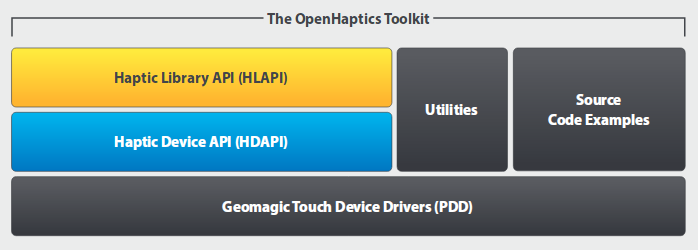
\includegraphics[scale=0.5,center]{openhaptics}
\caption{Architektura pakietu OpenHaptics}
\end{figure}

Składnia bibliotek programistycznych pakietu OpenHaptics Toolkit jest wzorowana na składni biblioteki OpenGL i umożliwia tworzenie programów w języku C oraz C++. 

\subsection{Phantom Device Drivers}
Producent oprócz Phantom Omni dostarcza także innego rodzaju urządzenia haptyczne, skierowane do innych grup odbiorców. Phantom Device Drivers (PDD) to zestaw sterowników do wszystkich urządzeń haptycznych oferowanych przez producenta. 

\subsection{Haptic Device API}
Haptic Device API (HDAPI) to niskopoziomowe interfejs programistyczny umożliwiający bezpośredni dostęp do wszystkich funkcji związanych z urzadzeniami haptycznymi.

Poniższy diagram przedstawia kompletną architekturę modułu HDAPI:

\begin{figure}[H]
\centering
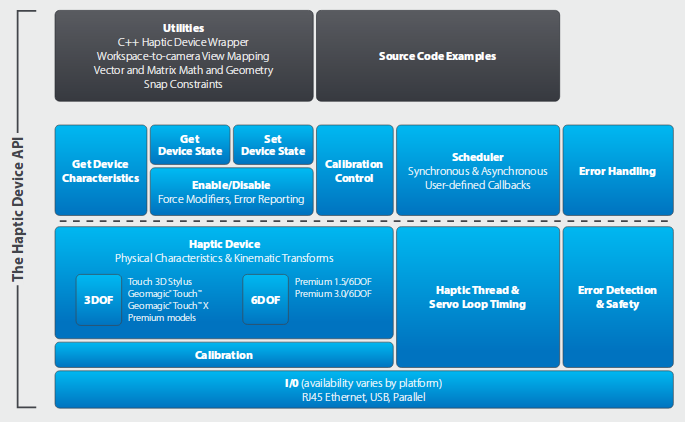
\includegraphics[scale=0.65,center]{hdapi}
\caption{Architektura HDAPI}
\end{figure}

Poza bardziej zaawansowanymi funkcjami związanymi na przykład z takimi aspektami jak wielowątkowość czy wywołania synchroniczne i asynchroniczne, HDAPI zwraca elementarne dane o pozycji i orientacji, umożliwia sterowanie sprzężeniem zwrotnym czy wyzwalanie funkcji (ang. callback) w odpowiedzi na wciskanie wbudowanych przycisków.

HDAPI dostarcza także rozbudowane API systemu detekcji i przechwytywania błędów, kalibracji urządzenia, itp.

Programista dostaje także bogaty zestaw przykładowych kodów źródłowych stanowiących przykłady wykorzystania poszczególnych funkcjonalności HDAPI.

\subsection{Haptic Library API}
Haptic Library API (HLAPI) to biblioteki wysokopoziomowego interfejsu programistycznego zaprojektowane głównie pod kątem zgodności z OpenGL API. HLAPI umożliwia dalekoidącą integrację z istniejącym kodem i \textit{bytami} (strukturami, funkcjami, itp.) pochodzącymi z OpenGL. Ponadto ułatwia współpracę z zewnętrznymi bibliotekami dostarczającymi funkcjonalności obliczeń fizycznych (dynamika, detekcji kolizji, itp.).

W odróżnieniu od surowego sterowania momentami sił działającymi na urządzenie (jak w przypadku HDAPI), tutaj możemy definiować bardziej złożone obiekty przestrzenne (bryły, powierzchnie) na które urządzenie haptyczne może oddziaływać. Również sposób reprezentacji sił dostarczony przez HLAPI jest bardziej rozbudowany, do dyspozycji programisty jest symulacja lepkości, sprężyny, grawitacji czy  tarcia.

Podobnie jak w przypadku HDAPI programista dostaje bogaty zestaw przykładowych kodów źródłowych, umożliwiających natychmiastowe przestestowanie interesujących rozwiązań.

Poniższy diagram przedstawia kompletną architekturę modułu HLAPI:

\begin{figure}[H]
\centering
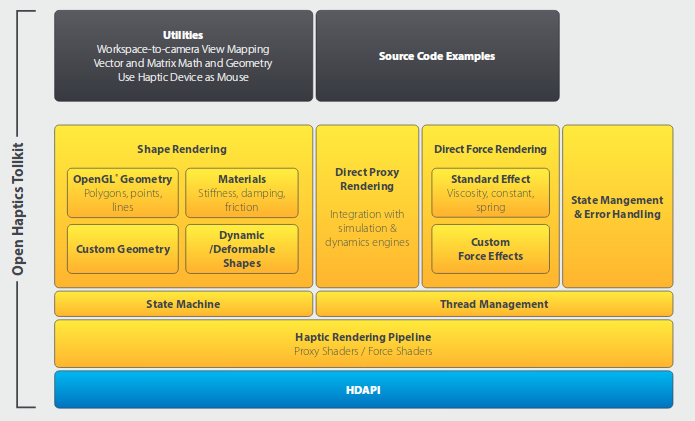
\includegraphics[scale=0.65,center]{hlapi}
\caption{Architektura HLAPI}
\end{figure}

\subsection{QuickHaptics Micro API}
QuickHaptics Micro API jest rozwiązaniem działającym \textit{na szczycie piramidy} OpenHaptics Toolkit.
\begin{figure}[H]
\centering
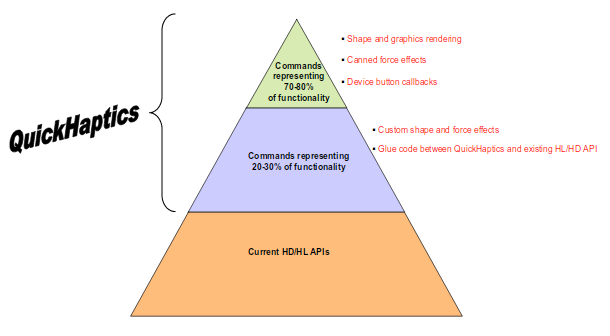
\includegraphics[scale=0.6,center]{quickhaptics}
\caption{QuickHaptics Micro API}
\end{figure}

Zgodnie z zapewnieniami producenta, QuickHaptics dostarcza jeszcze szybszych i łatwiejszych rozwiązań do tworzenia aplikacji wykorzystujących możliwości jego urządzeń. QuickHaptics Micro API stanowi kolejny, jeszcze wyższy poziom abstrakcji ponad HDAPI oraz HLAPI, który integrując je dostarcza interfejsy w postaci klas języka C++. Umożliwia tworzenie w pełni funkcjonalnych programów przez osoby nie posiadające dużego doświadczenia w zakresie metod wirtualnej rzeczywistości, programowania grafiki komputerowej czy obsługi urządzeń haptycznych.

Wszystkie elementy składające się na OpenHaptics Toolkit mogą być ze sobą łączone i używane zamiennie. 

\section{Servo Loop}
\textit{Servo Loop} to specjalna, działająca w osobnym wątku z wysokim priorytetem pętla, którą musi posiadać każdy program współpracujący z urządzeniami haptycznymi.

\begin{figure}[H]
\centering
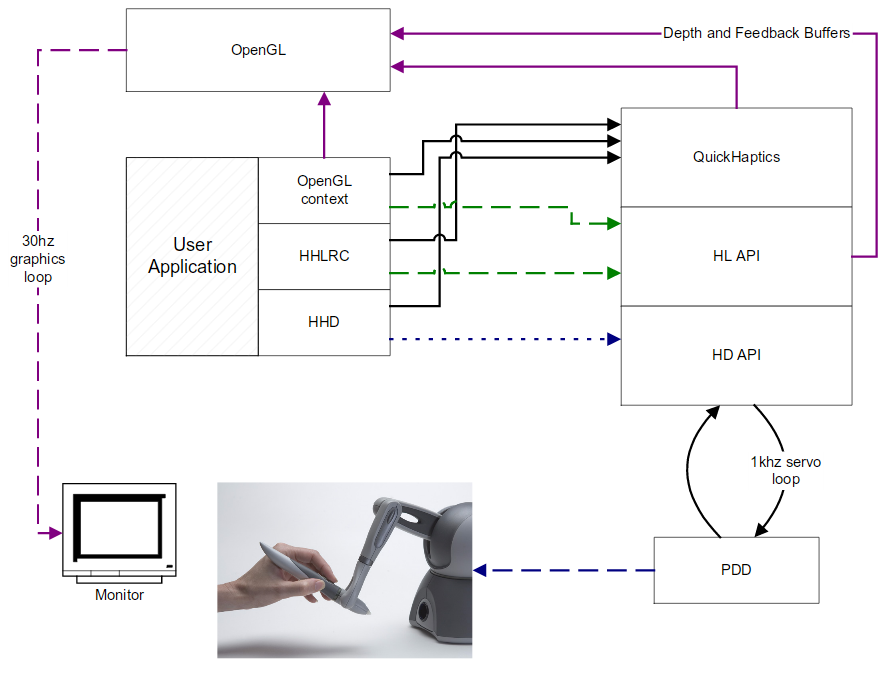
\includegraphics[scale=0.5,center]{servoloop}
\caption{Servo Loop}
\end{figure}

Zapewnienie stabilnego i realistycznego odwzorowania efektów sprzężenia zwrotnego jest tutaj najwyższym priorytetem. Wymagane jest aby pętla \textit{Servo Loop} była wykonywana z częstotliwością co najmniej 1kHz.

\chapter{Virtual Reality Peripheral Network}
Virtual Reality Peripheral Network (w skrócie VRPN) jest rozbudowaną biblioteką, szkieletem aplikacji (ang. application framework) i zbiorem narzędzi ułatwiających tworzenie programów komputerowych wykorzystujących urządzenia używane w systemach wirtualnej rzeczywistości. VRPN dostarcza abstrakcyjnych interfejsów programistycznych i serwerów uniezależniających programistę konkretnych rozwiązań sprzętowych. Umożliwia stosunkowo proste budowanie aplikacji obsługujących urządzenia HCI w wielu popularnych językach programowania (np. C++, Python czy Java) \cite{taylorHudsonSeegerWeber}.

\section{Opis pakietu}
Pakiet VRPN jest od podstaw zaprojektowany jako oprogramowanie sieciocentryczne, tzn. takie w którym sieć komputerowa odgrywa kluczową rolę.

\begin{figure}[H]
\centering
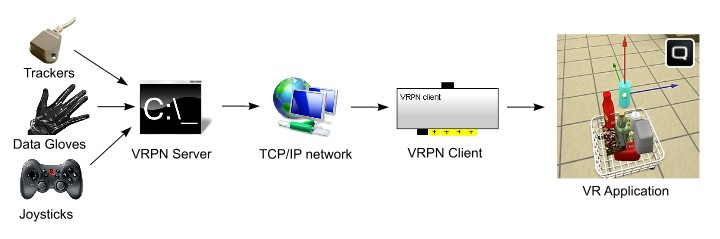
\includegraphics[scale=0.6,center]{vrpn}
\caption{Architektura VRPN}
\end{figure}

VRPN definiuje kilka abstrakcyjnych klas wspieranych urządzeń: Analog, Button, Dial, ForceDevice, Imager, Sound, Text oraz Tracker. Przy czym konkretne urządzenie może należeć jednocześnie do jednej lub kilku klas (np. Phantom Omni to Tracker, Button oraz ForceDevice). Istnienie ww. klas powoduje, że wszystkie urządzenia danego typu zgłaszają zmiany stanów jako asynchroniczne wywołania funkcji (ang. callback) przekazując w ten sposób obiekty lub wartości parametrów swoich klas. Zadaniem programisty jest odbiór i interpretacja przychodzących danych. Pozwala to na wygodne i szybkie wdrażanie rozwiązań opartych o urządzenia HCI nawet przez osoby bez wcześniejszego doświadczenia z systemami wirtualnej rzeczywistości.

Domyślnie VRPN jest napisany w języku C++, jednak posiada wbudowane mechanizmy generujące kod w języku Python czy Java. W trakcie kompilacji biblioteki z zamiarem jej użycia po stronie klienckiej należy zwrócic szczególną uwagę na docelowy język którego będziemy używać i podać odpowiednie parametry kompilacji. 

\section{Opis użycia VRPN}
W niniejszej pracy wykorzystuje się integrację pakietu VRPN z urządzeniem Phantom Omni do otrzymywania danych statusowych o pozycji, orientacji i wciśniętych przyciskach oraz sterowania sprzężeniem zwrotnym \cite{rodriguezGonzalez2015}.

Stacja robocza obsługująca urządzenie haptyczne posiada skonfigurowany do jego obsługi proces \textit{vrpn\_server} będący serwerem TCP/IP oczekującym na przychodzące połączenia od zainteresowanych aplikacji klienckich. Konfiguracja serwera jest przechowywana w tekstowym pliku konfiguracyjnym \textit{vrpn.cfg}, który jest ładowany każdorazowo podczas uruchamiania. 

Stworzona aplikacja, w tym przypadku wtyczka do programu PyMOL, jest klientem TCP/IP próbującym nawiązać połączenie z ww. serwerem. W trakcie jej uruchamiania tworzone są obiekty klas \textit{vrpn\_Tracker}, \textit{vrpn\_Button} i \textit{vrpn\_ForceDevice} posiadające wskaźniki do funkcji-uchwytów (ang. handler) odpowiednio przetwarzających odebrane danymi.

Zarejestrowanie funkcji-uchwytu (tutaj funkcja \textit{button\_handler(...)}) w obiekcie klasy \textit{vrpn\_Button} i obsługa przychodzących zdarzeń jest trywialna i sprowadza się do rozpoznania zmiany stanu jednego z dwóch przycisków. W ramach niniejszej pracy przyciski zostały oprogramowane tak, że wciśnięcie pierwszego z nich powoduje wykonanie superpozycji (nałożenia się) struktury wzorca z najbliższym możliwym do dopasowania regionem - zgodnie z danymi pochodzącymi z \textit{pliku mapującego}. Wciśnięcie drugiego przycisku powoduje wykonanie zbliżenia na linię łączącą środki ciężkości ww. struktur.

Dane udostępniane przez obiekt klasy \textit{vrpn\_Tracker} to pozycja i orientacja wskaźnika. Odebrane surowe dane należy przeliczyć na jednostki i wielkości obsługiwane przez pakiet PyMOL. W przypadku orientacji należy przejść z reprezentacji w kwaternionach (wydawana przez VRPN) na postać (akceptowaną przez PyMOL) oś-kąt (ang. axis-angle), ta operacja została opisana w części teoretycznej pracy. Współrzędne pozycji wskaźnika należy przemnożyć przez dobrany eksperymentalnie współczynnik skalujący, który spowoduje realistyczne odwzorowanie przesunięć z przestrzeni rzeczywistej w przestrzeni wirtualnej.

Klasa \textit{vrpn\_ForceDevice} umożliwia sterowanie serwomechanizmami wbudowanymi w urządzenie Phantom Omni. Biblioteka VRPN dostarcza szereg metod umożliwiających wykonanie takich operacji na kilka sposobów: począwszy od najprostszego podania wektora pola siłowego, poprzez zdefiniowanie wirtualnej sprężyny zaczepionej w zadanym punkcie, aż do tworzenia wirtualnych powierzchni czy brył.

Integracja oraz przetwarzanie danych dostarczanych przez pakiet VRPN były znaczącą częścią pracy. Użycie pakietu VRPN zamiast w miejsce biblioteki OpenHaptics dało znaczący wzrost niezależności projektu od konkretnego urządzenia haptycznego i otworzyło wiele możliwości dalszego rozwoju i wykorzystania stworzonego w ramach niniejszej pracy oprogramowania. 

\chapter{Implementacja i uruchomienie oprogramowania}

Oprogramowanie będące przedmiotem niniejszej pracy zostało stworzone jako rozszerzenie (ang. plugin) popularnego pakietu PyMOL. Wykorzystano w nim możliwości wizualizacyjne pakietu w połączeniu z danymi o pozycji i orientacji urządzenia Phantom Omni odbieranymi dzięki bibliotece VRPN. Dane wejściowe do programu - plik mapujący struktury biopolimerów - został dostarczony przez zewnętrzne oprogramowanie (opisane w części teoretycznej pracy).

\section{Opis stanowiska laboratoryjnego}
Jak wspomniano we wstępie do pracy prawidłowe uruchomienie oprogramowania będącego jej przedmiotem wymaga wcześniejszego zestwienia odpowiednio skonfigurowanego stanowiska laboratoryjnego. 

\begin{figure}[H]
\centering
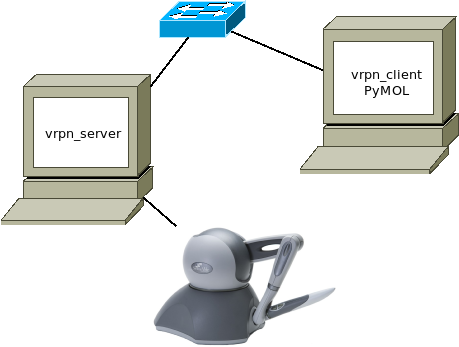
\includegraphics[scale=0.6,center]{stanowisko}
\caption{Schemat stanowiska laboratoryjnego}
\end{figure}

Stanowisko składa się z połączonych siecią komputerową stacji roboczych, gdzie jedna stanowi host urządzenia Phantom Omni, druga natomiast to łączący się z nią klient ze stworzonym oprogramowaniem. 

Komputer-host musi posiadać kompatybilną z urządzeniem Phantom Omni kartę rozszerzeń z portem IEEE-1394 (FireWire), sterowniki wraz z pakietem OpenHaptics oraz VRPN ze skonfigurowanym procesem \textit{vrpn\_server} nasłuchującym połączeń przychodzących na wybranym porcie TCP. 

Druga stacja robocza stanowiska laboratoryjnego posiada zainstalowany pakiet PyMOL z oprogramowaniem rozszerzającym jego funkcjonalność - przedmiotem niniejszej pracy. Po jego uruchomieniu, załadowaniu danych wejściowych oraz wprowadzeniu adresu sieciowego hosta urządzenia Phantom Omni, program próbuję nawiązać z nim połączenie i rozpocząć pracę.

W szczególności host urządzenia Phantom Omni oraz pakiet PyMOL mogą być uruchomione na jednej maszynie i wykorzystywać interfejs \textit{localhost}.

\section{Rozszerzanie funkcjonalności pakietu PyMOL}

PyMOL jest oprogramowaniem służącym głównie do wizualizacji struktur chemicznych oraz przeprowadzania na nich prostych obliczeń. Jego historia sięga roku 2000, kiedy to Warren Lyford DeLano zainicjował powstanie projektu. Przez lata intensywnych prac nad rozwojem program stał się standardowym narzędziem wykorzystywanym przez wiele wiodących ośrodków naukowo badawczych. Od roku 2010 nad jego rozwojem czuwa firma \textit{Schrödinger, Inc}.

Funkcjonalność pakiet PyMOL może być w łatwy sposób rozszerzalna poprzez wbudowany system obsługi wtyczek (ang. plugin) tworzonych w języku Python. Programista ma dostęp do rozbudowanego API (ang. application programming interface) zawierającego szeroki wachlarz funkcji umożliwiających tworzenie wizualizacji oraz obliczeń na załadowanych reprezentacjach struktur chemicznych. Ponadto programista tworząc wtyczki może z powodzeniem korzystać z biblioteki standardowej języka Python oraz dowolnych innych bibliotek pochodzących od zewnętrznych dostawców.

Podczas tworzenia niniejszego oprogramowania wykorzystano zarówno API wbudowane w PyMOL jak również pochodzące z zewnętrznych bibliotek takich jak VRPN do efektywnej obsługi urządzenia haptycznego.

Proces tworzenia wtyczek do pakietu PyMOL jest trywialny i został szczegółowo opisany w jego dokumentacji. 

\section{Dane wejściowe}
Oprogramowanie do poprawnego uruchomienia wymaga podania dwóch plików w formacie PDB (ang. protein data bank) oraz pliku mapującego. Pierwszy z nich zawiera główną strukturę biopolimeru (ang. target), drugi natomiast reprezentuje wzorcowy fragment (ang. template). Plik mapujący z kolei jest generowany przez zewnętrzne oprogramowanie.

\textit{Struktura celu} to najczęściej cała, duża cząsteczka białka lub kwasu nukleinowego, składająca się z setek lub tysięcy merów. W programie zostaje ona umieszczona w początku układu współrzędnych i jest nieruchoma względem wskaźnika urządzenia haptycznego.

\textit{Wzorcowy fragment} może stanowić krótki (najczęściej kilkanaście lub kilkadziesiąt merów) wycinek struktury celu lub dowolną inną podjednostkę czy fragment struktury drugorzędowej (np. $\alpha$-helisa). Zostaje on na stałe związany z ruchem wskaźnika urządzenia haptycznego. Każde jego przesunięcie czy zmiana orientacji zostaje w czasie rzeczywistym odwzorowana na ekranie. 

\textit{Plikiem mapującym} nazywamy dane uzyskane z obliczeń przeprowadzonych przez zewnętrzne oprogramowanie, zawierających informacje o takich regionach struktury celu, których stopień podobieństwa (dopasowania) do struktury wzorcowej nie przekracza zadanego progu. Dane te są kluczowe do działania niniejszego oprogramowania, gdyż na ich podstwie wyliczane są odległości i momenty sił projektowane do urządzenia Phantom Omni. Poza ozwierciedleniem odległości w urządzeniu haptycznym, na ekranie PyMOL wyświeltany jest odcinek łączący wzorcową strukturę z najbliższym optymalnie pasującym regionem struktury głównej.

\begin{figure}[H]
\centering

\includegraphics[scale=0.3,center]{todo}
\caption{Okno ładowania plików i danych wejściowych}
\end{figure}

\section{Opis oprogramowania}
Po zestawieniu i skonfigurowaniu stanowiska laboratoryjnego zgodnie z wcześniejszym opisem na komputerze będącym hostem urządzenia Phantom Omni należy uruchomić proces \textit{vrpn\_server}.

Na komputerze z oprogramowaniem PyMOL należy uruchomić zainstalowaną wtyczkę przez kliknięcie odpowiedniej pozycji w menu \textit{Plugin}.

\begin{figure}[H]
\centering

\includegraphics[scale=0.3,center]{todo}
\caption{Uruchamianie oprogramowania}
\end{figure}

W kolejnym kroku pojawi się ekran powitalny z krótkim opisem możliwości oferowanych przez oprogramowanie.

\begin{figure}[H]
\centering

\includegraphics[scale=0.3,center]{todo}
\caption{Ekran powitalny}
\end{figure}

Po kliknięciu na przycisk \textit{Dalej} przechodzimy do kolejnego okna, które daje nam możliwość przeglądania dysku w poszukiwaniu odpowiednich plików wejściowych. Ponadto należy podać adres komputera, na którym uruchomiony jest proces \textit{vrpn\_server}. W przypadku pracy na lokalnej maszynie w oknie należy podać adres \textit{phantom@127.0.0.1} lub \textit{phantom@localhost}.

\begin{figure}[H]
\centering

\includegraphics[scale=0.3,center]{todo}
\caption{Wprowadzanie danych wejściowych}
\end{figure}

Program zakłada poprawność wprowadzonych danych, tzn nie jest przeprowadzane sprawdzenie czy załadowane pliki są zgodne z formatem PDB czy prawidłowym formatem pliku mapującego.

W kolejnym kroku program próbuje nawiązać połączenie TCP z hostem i urządzeniem haptycznym. Prawidłowe nawiązanie połączenia rozpoczyna wymianę danych pomiędzy aplikacjami. Proces \textit{vrpn\_server} wysyła komunikaty o pozycji oraz orientacji wskaźnika, natomiast PyMOL za pośrednictwem sieci wysyła informację o sprzężeniu zwrotnym do urządzenia Phantom Omni. 

Na ekranie widać wzorcową strukturę poruszającą się zgodnie z ruchami urządzenia haptycznego, natomiast urządzenie haptyczne dostaje polecenia sterujące momentami sił, przyciągając wskaźnik do najbliższego (wskazywanego na ekranie przez biały odcinek) podobnego regionu w ramach struktury celu.

\begin{figure}[H]
\centering

\includegraphics[scale=0.3,center]{todo}
\caption{Ekran główny 1}
\end{figure}

\begin{figure}[H]
\centering

\includegraphics[scale=0.3,center]{todo}
\caption{Ekran główny 2}
\end{figure}

\begin{figure}[H]
\centering

\includegraphics[scale=0.3,center]{todo}
\caption{Ekran główny 3}
\end{figure}

\chapter{Perspektywy rozwoju i praktycznego wykorzystania}
Obecny poziom rozwoju stworzonego w ramach pracy oprogramowania pozwala na stosunkowo proste przeglądanie i dopasowywanie struktur chemicznych za pomocą wskaźnika haptycznego Phantom Omni. Wykorzystuje do tego dane wejściowe pochodzące z innych źródeł.

W obecnej formie oprogramowanie może mieć dość ograniczone zastosowanie praktyczne - np. w przemyśle - dość dobrze może jednak nadawać się do celów naukowo-edukacyjnych demonstrujących możliwości wykorzystania metod wirtualnej rzeczywistości w takich dziedzinach nauki jak biofizyka, biologia molekularna czy chemia.

Wykorzystanie integracji urządzenia Phantom Omni z pakietem VRPN i PyMOL w połączeniu z różnymi metodami bioinformatycznymi tworzy cały szereg nowych i być może nieznanych dotąd (lub niemających praktycznego wykorzystania) możliwości. Ławtość wchodzenia w interakcję z wykreowanym, wirtualnym, molekularnym światem i odzwierciedlanie sił obecnych na tym poziomie może znacznie ułatwić i rozszerzyć proces edukacji przyszłych adeptów ww. nauk. 

Dalszy rozwój niniejszego oprogramowania może polegać na dodaniu funkcjonalności, które w chwili obecnej realizuje oprogramowanie zewnętrzne. Wymagałoby to rozbudowy obecnego programu o część realizującą obliczenia dopasowań strukturalnych implementując różne ich metody. 

Kolejnym etapem rozszerzania funkcjonalności niniejszego oprogramowania mogłoby być dodanie metod bioinformatycznych związanych z dokowaniem molekularnym i projektowaniem leków.

W przypadku dalszego rozwoju funkcjonalności oprogramowania zgodnie z powyższymi lub innymi propozycjami możliwe jest wyobrażenie sobie wykorzystania tego oprogramowania na szerszą skalę w ośrodkach naukowo-badawczych uczelni lub przemysłu.

\chapter{Podsumowanie}

W ramach niniejszej pracy została przedstawiona implementacja oprogramowania, którego funkcjonalność obejmuje interaktywne przeglądanie struktur biopolimerów w poszukiwaniu regionów podobnych (z dokładnością do zadanego progu) do wybranej struktury wzorcowej. Oprogramowanie wykorzystuje metody i urządzenia wirtualnej rzeczywistości, w szczególności urządzenie haptyczne Phantom Omni oraz pakiet VRPN. Oprogramowanie powstało w formie wtyczki rozszerzającej funkcjonalność pakietu PyMOL, wykorzystując jego możliwości wizualizacji struktur chemicznych.

Zostały także przedstawione podstawy teoretyczne pracy, na które składały się globalne i lokalne metody dopasowania (uliniowienia) strukturalnego, algorytm RMSD służący do oceny ww. dopasowań oraz Kabsch'a - metoda minimalizująca wartość RMSD, maksymalizująca stopień dopasowania. Opisane także zostały elementarne przekształcenia geometryczne wykorzystywane w pracy oraz sposób konwersji kwaternionów na macierze rotacji (wykorzystywane przez pakiet PyMOL).

Szczegółowo zostało opisane urządzenie haptyczne Phantom Omni i jego integracja z pakietem Virtual Reality Peripheral Network.

W końcowej części została podana bibliografia, z której korzystano w trakcie tworzenia niniejszej pracy. 

Kod źródłowy stworzonego oprogramowania wraz z obszernymi komentarzami stanowi załącznik do niniejszego opracowania.

\iffalse
\chapter{Podstawowe pojęcia}\label{r:pojecia}

Pojęciem pierwotnym blabalii fetorycznej jest \emph{blaba}.
Blabaliści nie podają jego definicji, mówiąc za Ciach-Pfe t-\=am
K\^un (fooistyczny mędrzec, XIX w. p.n.e.):
\begin{quote}
  Blaba, który jest blaba, nie jest prawdziwym blaba.

\raggedleft\slshape tłum. z~chińskiego Robert Blarbarucki
\end{quote}

\section{Definicje}

Oto dwie definicje wprowadzające podstawowe pojęcia blabalii
fetorycznej:

\begin{defi}\label{skupienie}
  Silny, zwarty i gotowy fetor bazowy nazwiemy \emph{skupieniem}.
\end{defi}

\begin{defi}\label{fetor}
  \emph{Fetorem} nazwiemy skupienie blaba spełniające następujący
  \emph{aksjomat reperkusatywności}:
  $$\forall \mathcal{X}\in Z(t)\ \exists
  \pi\subseteq\oint_{\Omega^2}\kappa\leftrightarrow 42$$
\end{defi}


\section{Blabalizator różnicowy}

Teoretycy blabalii (zob. np. pracę~\cite{grglo}) zadowalają się
niekonstruktywnym opisem natury fetorów.

Podstawowym narzędziem blabalii empirycznej jest blabalizator
różnicowy.  Przyrząd ten pozwala w~sposób przybliżony uzyskać
współczynniki rozkładu Głombaskiego dla fetorów bazowych
i~harmonicznych.  Praktyczne znaczenie tego procesu jest oczywiste:
korzystając z~reperkusatywności pozwala on przejść do przestrzeni
$\Lambda^{\nabla}$, a~tym samym znaleźć retroizotonalne współczynniki
semi-quasi-celibatu dla klatek Rozkoszy (zob.~\cite{JR}).

Klasyczne algorytmy dla blabalizatora różnicowego wykorzystują:
\begin{enumerate}
\item dualizm falowo-korpuskularny, a w szczególności
  \begin{enumerate}
  \item korpuskularną naturę fetorów,
  \item falową naturę blaba,
  \item falowo-korpuskularną naturę gryzmołów;
  \end{enumerate}
\item postępującą gryzmolizację poszczególnych dziedzin nauki, w
  szczególności badań systemowych i rozcieńczonych;
\item dynamizm fazowy stetryczenia parajonizacyjnego;
\item wreszcie tradycyjne opozycje:
  \begin{itemize}
  \item duch --- bakteria,
  \item mieć --- chcieć,
  \item myśl --- owsianka,
  \item parafina --- durszlak\footnote{Więcej o tym przypadku --- patrz
      prace Gryzybór-Głombaskiego i innych teoretyków nurtu
      teoretyczno-praktycznego badań w~Instytucie Podstawowych
      Problemów Blabalii w~Fifie.},
  \item logos --- termos\footnote{Szpotański}
  \end{itemize}
  z właściwym im przedziwym dynamizmem.
\end{enumerate}

\begin{figure}[tp]
  \centering
  \framebox{\vbox to 4cm{\vfil\hbox to
      7cm{\hfil\tiny.\hfil}\vfil}}
  \caption{Artystyczna wizja blaba w~obrazie węgierskiego artysty
    Josipa~A. Rozkoszy pt.~,,Blaba''}
\end{figure}

\chapter{Wcześniejsze implementacje blabalizatora
  różnicowego}\label{r:losers}

\section{Podejście wprost}

Najprostszym sposobem wykonania blabalizy jest siłowe przeszukanie
całej przestrzeni rozwiązań.  Jednak, jak łatwo wyliczyć, rozmiar
przestrzeni rozwiązań rośnie wykładniczo z~liczbą fetorów bazowych.
Tak więc przegląd wszystkich rozwiązań sprawdza się jedynie dla bardzo
prostych przestrzeni lamblialnych.  Oznacza to, że taka metoda ma
niewielkie znaczenie praktyczne --- w~typowym przypadku z~życia trzeba
rozważać przestrzenie lamblialne wymiaru rzędu 1000.

W~literaturze można znaleźć kilka prób opracowania heurystyk dla
problemu blabalizy (por. \cite{heu}).  Korzystając z~heurystyk daje
się z~pewnym trudem dokonać blabalizy w~przestrzeni o~np.~500 fetorach
bazowych.  Należy jednak pamiętać, że heurystyka nie daje gwarancji
znalezienia najlepszego rozwiązania.  Fifak w~pracy~\cite{ff-sr}
podaje, jak dla dowolnie zadanej funkcji oceniającej skonstruować
dane, dla których rozwiązanie wygenerowane przez algorytm heurystyczny
jest dowolnie odległe od rzeczywistego.

\section{Metody wykorzystujące teorię Głombaskiego}

Teoria Głombaskiego (zob.~\cite{grglo}) dostarcza eleganckiego
narzędzia opisu przejścia do przestrzeni $\Lambda^{\nabla}$.
Wystarczy mianowicie przedstawić fetory bazowe wyjściowej przestrzeni
lamblialnej w~nieskończonej bazie tak zwanych wyższych aromatów.
(Formalną definicję tego pojęcia przedstawię w~rozdziale poświęconym
teorii Fifaka).  Podstawową cechą wyższych aromatów jest ulotność.  To
zaś oznacza, że odpowiednio dobierając współczynniki przejścia do
przestrzeni wyższych aromatów można zagwarantować dowolną z~góry
zadaną dokładność przybliżonego rozwiązania problemu blabalizy.

Oczywiście ze względu na nieskończony wymiar przestrzeni wyższych
aromatów koszt poszukiwania współczynników blabalizy jest liniowy ze
względu na wymiar wyjściowej przestrzeni lamblialnej.

\section{Metody wykorzystujące własności fetorów $\sigma$}

Najchętniej wykorzystywaną przestrzenią wyższych aromatów jest
przestrzeń fetorów~$\sigma$.  Fetory $\sigma$ dają szczególnie prostą
bazę podprzestrzeni widłowej.  Wiąże się to z~faktem, że w~tym przypadku
fetory harmoniczne wyższych rzędów są pomijalne (rzędu $2^{-t^3}$,
gdzie $t$ jest wymiarem wyjściowej przestrzeni lamblialnej).

Niestety z~fetorami $\sigma$ wiąże się też przykre ograniczenie: można
wykazać (zob.~\cite[s. 374]{ff-sr}), że dla dowolnie dobranej bazy
w~podprzestrzeni widłowej istnieje ograniczenie dolne w~metryce sierpa
na odległość rzutu dokładnego rozwiązania problemu blabalizy na
podprzestrzeń widłową.  Ponieważ rzut ten stanowi najlepsze
przybliżone rozwiązanie, jakie można osiągnąć nie naruszając aksjomatu
reperkusatywności, więc istnieje pewien nieprzekraczalny próg
dokładności dla blabalizy wykonanej przez przejście do przestrzeni
fetorów $\sigma$.  Wartość retroinicjalną tego progu nazywa się
\textit{reziduum blabicznym}.

\chapter{Teoria fetorów $\sigma$-$\rho$}\label{r:fifak}

Głównym odkryciem Fifaka jest, że fetor suprakowariantny może
gryzmolizować dowolny ideał w~podprzestrzeni widłowej przestrzeni
lamblialnej funkcji Rozkoszy.

Udowodnienie tego faktu wymagało wykorzystania twierdzeń pochodzących
z~kilku niezależnych teorii matematycznych (zob. na przykład:
\cite{russell,spyrpt,JR,beaman,hopp,srinis}).  Jednym z~filarów
dowodu jest teoria odwzorowań owalnych Leukocyta (zob.~\cite{leuk}).

Znaczenie twierdzenia Fifaka dla problemu blabalizy polega na tym, że
znając retroizotonalne współczynniki dla klatek Rozkoszy można
przeprowadzić fetory bazowe na dwie nieskończone bazy fetorów $\sigma$
w~przestrzeni $K_7$ i~fetorów $\rho$ w~odpowiedniej
quasi-quasi-przestrzeni równoległej (zob.~\cite{hopp}).  Zasadnicza
różnica w~stosunku do innych metod blabalizy polega na tym, że
przedstawienie to jest dokładne.

\chapter{Dokumentacja użytkowa i~opis implementacji}\label{r:impl}

Program przygotowany dla systemu operacyjnego M\$ Windows uruchamia
się energicznym dwumlaskiem na jego ikonce w~folderze
\verb+\\FIDO\FOO\BLABA+.  Następnie kolistym ruchem ręki należy
naprowadzić kursor na menu \texttt{Blabaliza} i~uaktywnić pozycję
\texttt{Otwórz plik}.  Po wybraniu pliku i~zatwierdzeniu wyboru
przyciskiem \texttt{OK} rozpocznie się proces blabalizy.  Wyniki
zostaną zapisane w~pliku o~nazwie \texttt{99-1a.tx.43} w~bieżącym
folderze.

\chapter{Podsumowanie}

W~pracy przedstawiono pierwszą efektywną implementację blabalizatora
różnicowego.  Umiejętność wykonania blabalizy numerycznej dla danych
,,z życia'' stanowi dla blabalii fetorycznej podobny przełom, jak dla
innych dziedzin wiedzy stanowiło ogłoszenie teorii Mikołaja Kopernika
i~Gryzybór Głombaskiego.  Z~pewnością w~rozpocznynającym się XXI wieku
będziemy obserwować rozkwit blabalii fetorycznej.

Trudno przewidzieć wszystkie nowe możliwości, ale te co bardziej
oczywiste można wskazać już teraz.  Są to:
\begin{itemize}
\item degryzmolizacja wieńców telecentrycznych,
\item realizacja zimnej reakcji lambliarnej,
\item loty celulityczne,
\item dokładne obliczenie wieku Wszechświata.
\end{itemize}

\section{Perspektywy wykorzystania w~przemyśle}

Ze względu na znaczenie strategiczne wyników pracy ten punkt uległ
utajnieniu.

\appendix

\chapter{Główna pętla programu zapisana w~języku T\=oFoo}

\begin{verbatim}
[[foo]{,}[[a3,(([(,),{[[]]}]),
  [1; [{,13},[[[11],11],231]]].
  [13;[!xz]].
  [42;[{,x},[[2],{'a'},14]]].
  [br;[XQ*10]].
 ), 2q, for, [1,]2, [..].[7]{x}],[(((,[[1{{123,},},;.112]],
        else 42;
   . 'b'.. '9', [[13141],{13414}], 11),
 [1; [[134,sigma],22]].
 [2; [[rho,-],11]].
 )[14].
 ), {1234}],]. [map [cc], 1, 22]. [rho x 1]. {22; [22]},
       dd.
 [11; sigma].
        ss.4.c.q.42.b.ll.ls.chmod.aux.rm.foo;
 [112.34; rho];
        001110101010101010101010101010101111101001@
 [22%f4].
 cq. rep. else 7;
 ]. hlt
\end{verbatim}

\chapter{Przykładowe dane wejściowe algorytmu}

\begin{center}
  \begin{tabular}{rrr}
    $\alpha$ & $\beta$ & $\gamma_7$ \\
    901384 & 13784 & 1341\\
    68746546 & 13498& 09165\\
    918324719& 1789 & 1310 \\
    9089 & 91032874& 1873 \\
    1 & 9187 & 19032874193 \\
    90143 & 01938 & 0193284 \\
    309132 & $-1349$ & $-149089088$ \\
    0202122 & 1234132 & 918324098 \\
    11234 & $-109234$ & 1934 \\
  \end{tabular}
\end{center}

\chapter{Przykładowe wyniki blabalizy
    (ze~współczynnikami~$\sigma$-$\rho$)}

\begin{center}
  \begin{tabular}{lrrrr}
    & Współczynniki \\
    & Głombaskiego & $\rho$ & $\sigma$ & $\sigma$-$\rho$\\
    $\gamma_{0}$ & 1,331 & 2,01 & 13,42 & 0,01 \\
    $\gamma_{1}$ & 1,331 & 113,01 & 13,42 & 0,01 \\
    $\gamma_{2}$ & 1,332 & 0,01 & 13,42 & 0,01 \\
    $\gamma_{3}$ & 1,331 & 51,01 & 13,42 & 0,01 \\
    $\gamma_{4}$ & 1,332 & 3165,01 & 13,42 & 0,01 \\
    $\gamma_{5}$ & 1,331 & 1,01 & 13,42 & 0,01 \\
    $\gamma_{6}$ & 1,330 & 0,01 & 13,42 & 0,01 \\
    $\gamma_{7}$ & 1,331 & 16435,01 & 13,42 & 0,01 \\
    $\gamma_{8}$ & 1,332 & 865336,01 & 13,42 & 0,01 \\
    $\gamma_{9}$ & 1,331 & 34,01 & 13,42 & 0,01 \\
    $\gamma_{10}$ & 1,332 & 7891432,01 & 13,42 & 0,01 \\
    $\gamma_{11}$ & 1,331 & 8913,01 & 13,42 & 0,01 \\
    $\gamma_{12}$ & 1,331 & 13,01 & 13,42 & 0,01 \\
    $\gamma_{13}$ & 1,334 & 789,01 & 13,42 & 0,01 \\
    $\gamma_{14}$ & 1,331 & 4897453,01 & 13,42 & 0,01 \\
    $\gamma_{15}$ & 1,329 & 783591,01 & 13,42 & 0,01 \\
  \end{tabular}
\end{center}

\fi

\begin{thebibliography}{99}
\addcontentsline{toc}{chapter}{Bibliografia}

\bibitem{anfinsen73} Christian B. Anfinsen, \textit{Principles that govern the folding of protein chains}, Science, 1973

\bibitem{casp} \textit{Critical Assessment of protein Structure Prediction}, http://predictioncenter.org/casproll/results.cgi

\bibitem{vrLecture2011} Paweł Daniluk, \textit{Metody wirtualnej rzeczywistości. Urządzenia haptyczne.}, Uniwersytet Warszawski, 2011 

\bibitem{daniluk11} Paweł Daniluk, \textit{Analiza podobieństwa struktur przestrzennych białek przy użyciu deskryptorów lokalnej struktury}, Uniwersytet Warszawski, 2011

\bibitem{kufarevaAbagyan2012} Irina Kufareva, Ruben Abagyan, \textit{Methods of protein structure comparison}, Methods in Molecular Biology, 2012

\bibitem{zhangSkolnick2005} Yang Zhang, Jeffrey Skolnick, \textit{TM-align: a protein structure alignment algorithm based on the TM-score}, Nucleic Acids Research, 2005

\bibitem{kabsch1976} Wolfgang Kabsch, \textit{A solution for the best rotation to relate two sets of vectors}, Acta Crystallographica, 1976

\bibitem{kabsch1978} Wolfgang Kabsch, \textit{A discussion of the solution for the best rotation to relate two sets of vectors}, Acta Crystallographica, 1978

\bibitem{vanDam2000} Andries van Dam, \textit{How Are Geometric
Transformations (T,R,S) Used in Computer Graphics?}, Introduction to computer graphics, 2000

\bibitem{magarshak1992} Y. Magarshak, \textit{Quaternion representation of RNA sequences and tertiary structures}, BioSystems, 1993

\bibitem{hamilton1843} William Hamilton, \textit{On Quaternions; or on a new System of Imaginaries in Algebra}, list do Johna T. Graves'a, 1843

\bibitem{geomagicTouchBrochure} 3D Systems, \textit{Haptic Devices. Haptic devices that add the sense of Touch to your digital world}

\bibitem{openHapticsBrochure} 3D Systems, \textit{OpenHaptics Developer Edition}, Broszura informacyjna producenta

\bibitem{openHapticsProgrammersGuide} 3D Systems, \textit{OpenHaptics Toolkit version 3.0 Programmers Guide}, przewodnik programisty, 2015

\bibitem{taylorHudsonSeegerWeber} Russell M. Taylor II, Thomas C. Hudson, Adam Seeger, Hans Weber, Jeffrey Juliano, Aron T. Helser, \textit{VRPN: A Device-Independent, Network-Transparent VR Peripheral System}, University of North Carolina, 2001

\bibitem{rodriguezGonzalez2015} M. Cuevas-Rodriguez, D. Gonzalez-Toledo, L. Molina-Tanco, A. Reyes-Lecuona, \textit{Contributing to VRPN with a new server for haptic devices}, University of Malaga, 2015

\end{thebibliography}

\chapter*{Kod źródłowy}
\addcontentsline{toc}{chapter}{Kod źródłowy}

todo: tu będzie kod źródłowy

\end{document}


%%% Local Variables:
%%% mode: latex
%%% TeX-master: t
%%% coding: latin-2
%%% End:
